\documentclass[11pt]{book}

%\usepackage{lnote}

\usepackage{CJKutf8,CJKnumb}
%\usepackage{CJKpunct} %a homemade package

\usepackage{fancyhdr}
\usepackage{titlesec}

\usepackage{indentfirst}
\usepackage{paralist}
\usepackage{verbatim}

\usepackage[plain]{fancyref}
\usepackage[bookmarksnumbered,dvipdfmx,unicode, pdfborder=1,breaklinks,colorlinks,linkcolor=RoyalBlue3,urlcolor=blue]{hyperref}
\usepackage{makeidx}

\usepackage{mflogo,texnames}
\usepackage{textcomp}

\usepackage{amsmath,amsfonts,amsthm}

\usepackage[x11names]{xcolor} %must before tikz, x11names defines RoyalBlue3
\usepackage{graphicx}
%\usepackage{ps4pdf} %conflict with tabularx
\usepackage{pstricks,pst-plot,pst-eps}
\usepackage{subfig}
\def\pgfsysdriver{pgfsys-dvipdfmx.def} %put before tikz
\usepackage{tikz}

\usepackage{booktabs,tabularx,multirow,colortbl,longtable}

\usepackage{chapterbib}
\usepackage[sectionbib,super,square,sort&compress]{natbib}


%中文设置
\newcommand{\song}{\CJKfamily{usong}}
\newcommand{\fang}{\CJKfamily{ufang}}
\newcommand{\kai}{\CJKfamily{ukai}}
\newcommand{\hei}{\CJKfamily{uhei}}

%\AtBeginDvi{\special{pdf:tounicode GBK-EUC-UCS2}} %not necessary if use UTF8.

%行距
\renewcommand{\baselinestretch}{1.25}

%页眉页脚
\pagestyle{fancy}
\fancyhf{}
\fancyhead[LE,RO]{\thepage}
\fancyhead[RE]{\leftmark}
\fancyhead[LO]{\rightmark}
\fancypagestyle{plain}{%设置plain页格式
    \fancyhf{}
    \renewcommand{\headrulewidth}{0pt}
}

%章节
\renewcommand{\chaptername}{第\CJKnumber{\thechapter}章}
\newcommand{\sectionname}{节}
\renewcommand{\figurename}{图}
\renewcommand{\tablename}{表}
\renewcommand{\bibname}{参考文献}
\renewcommand{\contentsname}{目~录}
\renewcommand{\listfigurename}{图~目~录}
\renewcommand{\listtablename}{表~目~录}
\renewcommand{\indexname}{索~引}
\titleformat{\chapter}[block]{\center\Huge}{\chaptername}{20pt}{}

\makeindex

%空白页
\makeatletter
\def\cleardoublepage{
    \clearpage\if@twoside\ifodd\c@page\else
    \hbox{}
    \vspace*{\fill}
    \begin{center}
        看什么看,没见过空白页?
    \end{center}
    \vspace{\fill}
    \thispagestyle{empty}
    \newpage
    \if@twocolumn\hbox{}\newpage\fi\fi\fi
}
\makeatother

%Code demo
\makeatletter
\newenvironment{mycode}{
    \noindent
    \newsavebox{\mybox}
    \begin{lrbox}{\mybox}
    \begin{minipage}[c]{.945\textwidth}
    \begin{verbatim}
}{
    \end{verbatim}
    \end{minipage}
    \end{lrbox}%
    \setlength{\fboxsep}{8pt}
    \colorbox{demo@bgcolor}{\usebox{\mybox}}
    \setlength{\fboxsep}{\oldfboxsep}
}

\newenvironment{myoutput}{
    \noindent
    \begin{lrbox}{\@tempboxa}
    \begin{minipage}[c]{.945\textwidth}
}{
    \end{minipage}
    \end{lrbox}%
    \setlength{\fboxsep}{8pt}
    \fbox{\usebox{\@tempboxa}}
    \setlength{\fboxsep}{\oldfboxsep}
}
\makeatother


\definecolor{demo@bgcolor}{gray}{.8}
\let\oldfboxsep\fboxsep
\newwrite\file
\newsavebox{\mybox}

\makeatletter
\def\demo@start{
    \begingroup% Lets Keep the Changes Local
    \@bsphack
    \immediate\openout \file \jobname.exa
    \let\do\@makeother\dospecials
    \catcode`\^^M\active
    \def\verbatim@processline{
        \immediate\write\file{\the\verbatim@line}
    }
    \verbatim@start
}

\def\demo@end{\immediate\closeout\file\@esphack\endgroup}

\def\demo@code#1#2{%
    \setlength{\fboxsep}{8pt}%
    \colorbox{#1}{%
    \begin{minipage}[c]{#2}
        \setlength{\fboxsep}{\oldfboxsep}
        \small\verbatiminput{\jobname.exa}
    \end{minipage}%
    }%
}

\def\demo@out#1{%
    \setlength{\fboxsep}{8pt}%
    \fbox{%
    \begin{minipage}[c]{#1}
        \setlength{\fboxsep}{\oldfboxsep}
        \small\input{\jobname.exa}
    \end{minipage}%
    }%
}

\newenvironment{code}{
    \demo@start
}{
    \demo@end
    \list{}{\itemindent-\leftmargin}
    \item
    \demo@code{demo@bgcolor}{.95\textwidth}
    \endlist
}

\newenvironment{halfcode}{
    \demo@start
}{
    \demo@end
    \list{}{\itemindent-\leftmargin}
    \item
    \demo@code{demo@bgcolor}{.52\textwidth}
    \endlist
}

\newenvironment{out}{
    \demo@start
}{
    \demo@end
    \list{}{\itemindent-\leftmargin}
    \item
    \demo@out{.95\textwidth}
    \endlist
}

\newenvironment{demo}{
    \demo@start
}{
    \demo@end
    \list{}{\itemindent-\leftmargin}
    \item
    \makebox[\textwidth][c]{%
        \demo@code{demo@bgcolor}{.52\textwidth}%
        \hspace{10pt}%
        \demo@out{.36\textwidth}%
    }
    \endlist
}

\newenvironment{fdemo}[1]{
    \begin{lrbox}{\mybox}%
    \setlength{\fboxsep}{8pt}%
    \fbox{%
    \begin{minipage}[c]{.36\textwidth}
        \setlength{\fboxsep}{\oldfboxsep}
        \small{#1}
    \end{minipage}%
    }%
    \end{lrbox}
    \demo@start
}{
    \demo@end
    \list{}{\itemindent-\leftmargin}
    \item
    \makebox[\textwidth][c]{%
        \demo@code{demo@bgcolor}{0.52\textwidth}%
        \hspace{10pt}%
        \usebox{\mybox}%
    }
    \endlist
}
\makeatother

\def\reflect#1{{\setbox0=\hbox{#1}\rlap{\kern0.5\wd0
  \special{x:gsave}\special{x:scale -1 1}}\box0 \special{x:grestore}}}
\def\XeTeX{\leavevmode
  \setbox0=\hbox{X\lower.5ex\hbox{\kern-.15em\reflect{E}}\kern-.1667em \TeX}%
  \dp0=0pt\ht0=0pt\box0 }

%图形设置
\DeclareGraphicsExtensions{.eps,.mps,.pdf,.jpg,.png}

\usetikzlibrary{arrows,decorations,positioning}
\pgfsetxvec{\pgfpoint{10pt}{0}}
\pgfsetyvec{\pgfpoint{0}{10pt}}
\tikzset{
    box/.style={rectangle,rounded corners=6pt, 
        minimum width=40pt, minimum height=20pt, inner sep=6pt,
        draw=gray,thick,fill=lightgray},
    arrow/.style={->, shorten >=1pt, >=stealth', semithick},
    larrow/.style={->, shorten >=1pt, >=stealth', semithick},
    bloop/.style={semithick, to path={-- ++(0,-35pt) -| (\tikztotarget)}},
    rloop/.style={semithick, to path={-- ++(10pt,0) |- (\tikztotarget)}}
}

\begin{document}
\begin{CJK*}{UTF8}{usong}
\CJKindent %can only be used in the CJK environment
\CJKtilde

\frontmatter

\title{\Huge\LaTeX~ Notes v~1.20}
\author{Alpha Huang\footnote{\url{http://www.dralpha.com/}}}
\date{2008年7月26日}
\maketitle


%\setcitestyle{numbers,square}

%前言页眉
\renewcommand{\chaptermark}[1]{\markboth{#1}{}}

% This is part of the book TeX for the Impatient.
% Copyright (C) 2003 Paul W. Abrahams, Kathryn A. Hargreaves, Karl Berry.
% See file fdl.tex for copying conditions.

\input macros
\frontchapter{前言}

{\tighten
Donald Knuth 開發的計算機排版系統 \TeX, 
提供了幾乎所有排版高質量數學符號和普通文本的功能.
它因為它獨有的易用性, 超羣的分詞處理和美觀的斷行而聞名天下.
因為這些非凡的功能, \TeX\ 已經成為數學, 自然科學, 工程領域領先的排版系統, 
並且被美國數學學會定為標準. 
同時, 它的成對軟件, ^{\Metafont}, 可以用來設計任意的字體, 尤其是數學排版所需要的符號.
\TeX\ 和 \Metafont\ 在科學和工程領域有很廣泛的應用, 
也被移殖到各種不同的計算機架構上.
\TeX 當然不是全能的, 它缺少對於圖片的完整支持, 
同時一些功能, 比如修訂線, 在 \TeX\ 中實現起來也比較麻煩.
但是, 這些缺點和它的優點比較起來, 是微不足道的.
\par}

\thisbook\/ 是為科學工作者, 數學工作者和專業排印者而寫的.
對於這些人而言, \TeX\ 不是一個興趣愛好, 而是一個非常有用的工具.
本書同時也面向那些對 \TeX\ 有很強烈興趣的計算機行業工作者.
我們希望不管是新手們還是熟悉 \TeX\ 的人, 都能從本書獲益.
我們假定我們的讀者羣體己經熟悉了基本的計算機操作, 
並且他們希望用最快的速度得到他們想要的信屲.
因此, 我們的目標是提供簡明的信息, 並且讓讀者能夠方便地獲取它們.

{\tighten This book therefore provides a bright searchlight, a stout
walking-stick, and detailed maps for exploring and using \TeX.  It will
enable you to master \TeX\ at a rapid pace through inquiry and
experiment, but it will not lead you by the hand through the entire
\TeX\ system.  Our approach is to provide you with a handbook for \TeX\
that makes it easy for you to retrieve whatever information you need.
We explain both the full repertoire of \TeX\ commands and the concepts
that underlie them.  You won't have to waste your time plowing through
material that you neither need nor want.  \par}

In the early sections we also provide you with enough orientation so
that you can get started if you haven't used \TeX\ before.  We assume
that you have access to a \TeX\ implementation and that you know how to
use a text editor, but we don't assume much else about your background.
Because this book is organized for ready reference, you'll continue to
find it useful as you become more familiar with \TeX.  If you prefer to
start with a carefully guided tour, we recommend that you first read
Knuth's ^{\texbook} (see \xrefpg{resources} for a citation), passing
over the ``dangerous bend'' sections, and then return to this book for
additional information and for reference as you start to use \TeX.  (The
dangerous bend sections of \texbook\ cover advanced topics.)

The structure of \TeX\ is really quite simple: a \TeX\ input document
consists of ordinary text interspersed with commands that give \TeX\
further instructions on how to typeset your document.  Things like math
formulas contain many such commands, while expository text contains
relatively few of them.

The time-consuming part of learning \TeX\ is learning the commands and
the concepts underlying their descriptions.  Thus we've devoted most of
the book to defining and explaining the commands and the concepts.
We've also provided examples showing \TeX\ typeset output and the
corresponding input, hints on solving common problems, information about
error messages, and so forth.  We've supplied extensive cross-references
by page number and a complete index.

We've arranged the descriptions of the commands so that you can look
them up either by function or alphabetically.  The functional
arrangement is what you need when you know what you want to do but you
don't know what command might do it for you.  The alphabetical arrangement
is what you need when you know the name of a command but you don't know exactly
what it does.

We must caution you that we haven't tried to provide a complete
definition of \TeX.  For that you'll need ^{\texbook}, which is the
original source of information on \TeX.  \texbook\ also contains a lot
of information about the fine points of using \TeX, particularly on the
subject of composing math formulas.  We recommend it highly.

In 1989 Knuth made a major revision to \TeX\ in order to adapt it to
$8$-bit character sets, needed to support typesetting for languages
other than English.  The description of \TeX\ in this book incorporates
that revision (see \xref{newtex}).

{\tighten 你可能正在使用一個專門的 \TeX\ 封裝形式, 
比如 ^{\LaTeX} 或者 ^{\AMSTeX} (見 \xref{resources}).
雖然這些封裝形式是完整的, 你仍可能為更好地控製 \TeX\ 而去使用 \TeX\ 本身獨有的一些功能, 
你可以使用這本書來學習你想要知道的這些功能, 
而把其它你不感興趣的東西扔在一邊.\par}

Two of us (K.A.H. and K.B.) were generously supported by the
University of Massachusetts at Boston during the preparation of this
book.  In particular, Rick Martin kept the machines running, and
Robert~A. Morris and Betty O'Neil made the machines available.  Paul
English of Interleaf helped us produce proofs for a cover design.

We wish to thank the reviewers of our book: Richard Furuta of the
University of Maryland, John Gourlay of Arbortext, Inc., Jill Carter
Knuth, and Richard Rubinstein of the Digital Equipment Corporation. We
took to heart their perceptive and unsparing criticisms of the original
manuscript, and the book has benefitted greatly from their insights.

We are particularly grateful to our editor, Peter Gordon of
Addison-Wesley.  This book was really his idea, and throughout its
development he has been a source of encouragement and valuable
advice.  We thank his assistant at Addison-Wesley, Helen Goldstein, for
her help in so many ways, and Loren Stevens of Addison-Wesley for her
skill and energy in shepherding this book through the production
process.  Were it not for our copyeditor, Janice Byer, a number of small
but irritating errors would have remained in this book.  We appreciate
her sensitivity and taste in correcting what needed to be corrected
while leaving what did not need to be corrected alone.  Finally, we wish
to thank Jim Byrnes of Prometheus Inc. for making this collaboration
possible by introducing us to each other.
\vskip1.5\baselineskip

\line{\it Deerfield, Massachusetts\hfil\rm P.\thinspace W.\thinspace A.}
\line{\it Manomet, Massachusetts\hfil\rm K.\thinspace A.\thinspace H.,
       K.\thinspace B.}

\vskip2\baselineskip

\noindent {\bf Preface to the free edition:} This book was originally
published in 1990 by Addison-Wesley.  In 2003, it was declared out of
print and Addison-Wesley generously reverted all rights to us, the
authors.  We decided to make the book available in source form, under
the GNU Free Documentation License, as our way of supporting the
community which supported the book in the first place.  See the
copyright page for more information on the licensing.

The illustrations which were part of the original book are not included
here.  Some of the fonts have also been changed; now, only
freely-available fonts are used.  We left the cropmarks and galley
information on the pages, to serve as identification.  An old version of
Eplain was used to produce it; see the {\tt eplain.tex} file for
details.

We don't plan to make any further changes or additions to the book
ourselves, except for correction of any outright errors reported to us,
and perhaps inclusion of the illustrations.

Our distribution of the book is at {\tt
ftp://tug.org/tex/impatient}.  You can reach us by email at {\tt
impatient@tug.org}.

\pagebreak
\byebye

\tableofcontents

\mainmatter
%正文页眉
\renewcommand{\chaptermark}[1]{\markboth{\chaptername\ #1}{}}
\renewcommand{\sectionmark}[1]{\markright{\thesection\ #1}}

\chapter{简介}

\begin{quotation}
滚滚长江东逝水,浪花淘尽英雄。是非成败转头空。青山依旧在,几度夕阳红。

白发渔樵江渚上,惯看秋月春风。一壶浊酒喜相逢。古今多少事,都付笑谈中。
\begin{flushright}
---~杨慎《临江仙》
\end{flushright}
\end{quotation}

\section{历史回顾}

\LaTeX~是一种面向数学和其它科技文档的电子排版系统。一般人们提到的~\LaTeX~是一个总称,它包括~\TeX、\LaTeX、\AmS-\LaTeX~等\footnote{一般认为~\TeX~是一种引擎,\LaTeX~是一种格式,而~\AmS-\LaTeX~等是宏集。此处目的是简介,故不展开讨论。}。

\TeX~的开发始于~1977~年~5~月,Donald E. Knuth\footnote{斯坦福大学计算机系教授,已退休。}开发它的初衷是用于《The Art of Computer Programming》的排版。1962~年~Knuth~开始写一本关于编译器设计的书,原计划是~12~章的单行本。不久~Knuth~觉得此书涉及的领域应该扩大,于是越写越多,如滔滔江水连绵不绝,又如黄河泛滥一发不可收拾。1965~年完成的初稿居然有~3000~页,全是手写的!据出版商估计,这些手稿印刷出来需要~2000~页,出书的计划只好改为七卷,每卷一或两章。1976~年~Knuth~改写第二卷的第二版时,很郁闷地发现第一卷的铅版不见了,而当时电子排版刚刚兴起,质量还差强人意。于是~Knuth~仰天长啸:“我要扼住命运的咽喉”,决定自己开发一个全新的系统,这就是~\TeX。

1978~年~\TeX~第一版发布后好评如潮,Knuth~趁热打铁在~1982~年发布了第二版。人们现在使用的~\TeX~基本就是第二版,中间只有一些小的改进。1990~年~\TeX~ v3.0~发布后,Knuth~宣布除了修正~bug~外停止~\TeX~的开发,因为他要集中精力完成那本巨著的后几卷\footnote{已出版的前三卷是:《Fundamental Algorithms》、《Seminumerical Algorithms》、《Sorting and Searching》;第四卷《Combinatorial Algorithms》和第五卷《Syntactic Algorithms》正在写作中,预计~2015~年出版;第六卷《Theory of Context-free Languages》和第七卷《Compiler Techniques》尚未安排上工作日程。}。此后每发布一个修正版,版本号就增加一位小数,使得它趋近于$\pi$(目前是~3.141592)。Knuth~希望将来他离世时,\TeX~的版本号永远固定下来,从此人们不再改动他的代码。他开发的另一个软件~\MF~也作类似处理,它的版本号趋近于$e$,目前是~2.71828。

\TeX~是一种语言也是一个宏处理器,这使得它很好很强大,但是它同时又很繁琐,让人难以接近。因此~Knuth~提供了一个对~\TeX~进行了封装的宏集~Plain \TeX,里面有一些高级命令,有了它最终用户就无须直接面对枯燥无味的~\TeX。

然而~Plain \TeX~还是不够高级,所以~Leslie Lamport\footnote{现供职于微软研究院。}在~80~年代初期开发了另一个基于~\TeX~的宏集~\LaTeX。1992~年~\LaTeX~ v2.09~发布后,Lamport~退居二线,之后的开发活动由~Frank Mittelbach~领导的~The LaTeX Team~接管。此小组发布的最后版本是~1994~年的~\LaTeXe,他们同时还在进行~\LaTeX~3~的开发,只是正式版看起来遥遥无期。

起初,美国数学学会(American Mathematical Society,AMS)看着\TeX~是好的,就派~Michael Spivak~写了~\AmS-\TeX,这项基于~Plain \TeX~的开发活动进行了两年(1983--1985)。后来与时俱进的~AMS~又看着~\LaTeX~是好的,就想转移阵地,但是他们的字体遇到了麻烦。恰好~Mittelbach~和~Rainer Schöpf(后者也是~LaTeX Team~的成员)刚刚发布了~New Font Selection Scheme for \LaTeX(NFSS),AMS~看着还不错,就拜托他们把~AMSFonts加入~\LaTeX,继而在~1989~年请他们开发~\AmS-\LaTeX。\AmS-\LaTeX~发布于~1990~年,之后它被整合为~\AmS~宏包,像其它宏包一样可以直接运行于~\LaTeX。

\section{优点和缺点}
当前的文字处理系统大致可以分为两种:标记语言(Markup Language)式的,比如\LaTeX;所见即所得(WYSIWYG)式的,比如~MS Word\footnote{其实~Word~也有自己的标记语言域代码(field code),只是一般用户不了解。}。

一般而言,\LaTeX~相对于所见即所得系统有如下优点:
\begin{itemize}
    \item 高质量\ 它制作的版面看起来更专业,数学公式尤其赏心悦目。
    \item 结构化\ 它的文档结构清晰。
    \item 批处理\ 它的源文件是文本文件,便于批处理,虽然解释(parse)源文件可能很费劲。
    \item 跨平台\ 它几乎可以运行于所有电脑硬件和操作系统平台。
    \item 免费\ 多数~\LaTeX~软件都是免费的,虽然也有一些商业软件。
\end{itemize}

相应地,\LaTeX~的工作流程、设计原则,资源的缺乏,以及开发人员的历史局限性等种种原因也导致了一些缺陷:
\begin{itemize}
    \item 制作过程繁琐,有时需要反复编译,不能直接或实时看到结果。
    \item 宏包鱼龙混杂,水准参差不齐,风格不够统一。
    \item 排版风格比较统一,但因而缺乏灵活性。
    \item 用户支持不够好,文档不完善。
    \item 对国际语言和字体的支持很差。
\end{itemize}

抛开~MS Word~不谈,即使跟同为标记语言的~HTML/Web~系统相比,\LaTeX~也有一些不足之处。比如~Web~浏览器对~HTML~内容的渲染(render)比~DVI~浏览器对~\LaTeX~内容的渲染要快上许多,基本上可以算是实时。虽然~HTML~内容可能没有~LaTeX~那么复杂,但是~DVI~毕竟是已经被~\LaTeX~编译过的格式。

还有一点令人困惑的是,有一部分~\LaTeX~阵营的人士习惯于称对方为“邪恶的”或“出卖灵魂的”,如果昂贵的微软系统应当为人诟病,那么更贵的苹果系统为何却被人追捧?

2000~年有记者在采访~Lamport~时问:“为什么当前没有高质量的所见即所得排版系统?”他回答道:“门槛太高了,一个所见即所得系统要做到~\LaTeX~当前的水平,工作量之大不是单枪匹马所能完成\footnote{\TeX/\LaTeX~也不单单是那几个大腕儿完成的,他们背后还有众多默默无闻的小人物,比如当年~Knuth~手下的大批学生。此所谓一将功成万骨枯。}。微软那样的大公司可以做,但是市场太小了。我偶尔也会想加入“Dark Side”,让微软给我一组人马来开发一个这样的系统。”(包老师注:他果然于次年加入微软。)

窃以为这两大阵营其实是萝卜青菜的关系,与其抱残守缺、互相攻讦,不如各取所需;甚至可以捐弃前嫌、取长补短,共建和谐社会。

\section{软件准备}
\label{sec:latexsoft}

\LaTeX~是一个软件系统,同时也是一套标准。遵照这些标准,实现了(implement)所要求功能的软件集合被称为发行版(distribution)。与此类似的例子有~Java~和~Linux,比如SUN、IBM、BEA~等公司都有自己的~Java~虚拟机(JVM),它们都被称作~Java~的实现;而Linux~有~Red Hat/~Fedora、Ubuntu、SuSE~等众多的发行版。

\begin{table}[htbp]
\caption{\LaTeX~发行版与编辑器}
\label{tab:latexsoft}
\centering
\begin{tabular}{lll}
    \toprule
    操作系统 & 发行版 & 编辑器 \\
    \midrule
    Windows & \href{http://www.miktex.org/}{MikTeX} & \href{http://www.toolscenter.org/}{TeXnicCenter}、\href{http://www.winedt.com/}{WinEdt} \\
    Unix/Linux & \href{http://www.tug.org/texlive/}{TeX Live} & \href{http://www.gnu.org/software/emacs/emacs.html}{Emacs}、\href{http://vim.sourceforge.net/}{vim}、\href{http://kile.sourceforge.net/}{Kile} \\
    Mac OS & \href{http://www.tug.org/mactex/}{MacTeX} & \href{http://www.uoregon.edu/~koch/texshop/}{TeXShop} \\
    \bottomrule
\end{tabular}
\end{table}

\LaTeX~发行版只提供了一个~\LaTeX~后台处理机制,用户还需要一个前台编辑器来编辑它的源文件。常用的~\LaTeX~发行版和编辑器见\fref{tab:latexsoft}。在使用~\LaTeX~的过程中可能还需要其它一些软件,将在后面相关章节中分别介绍。

\section{学习方法}
\begin{quotation}
在科学上没有平坦的大道,只有那些不畏劳苦沿着陡峭山路攀登的人,才有希望达到光辉的顶点。
\begin{flushright}
---~卡尔·马克思
\end{flushright}
\end{quotation}

\begin{quotation}
无他,唯手熟尔。
\begin{flushright}
---~卖油翁
\end{flushright}
\end{quotation}

\begin{quotation}
用心。
\begin{flushright}
---~斯蒂芬·周
\end{flushright}
\end{quotation}

限于篇幅和水平,本文只能提供一个概览外加一些八卦。比较严谨的入门资料有~Tobias Oetiker~的《A (Not So) Short Introduction to \LaTeXe》\citep{Oetiker_2008}(简称lshort);若想对~\LaTeX~有更深入全面的了解,可以拜读~Mittelbach~的《The \LaTeX~ Companion》\citep{Mittelbach_2004}。

中文资料可参考李果正的《大家来学~\LaTeX》\citep{Lee_2004},lshort~有吴凌云等人翻译的中文版本\footnote{此译本首发于~CTeX~论坛,但是需要注册才能看见链接,所以请读者自行搜索。}。

\href{http://www.ctan.org/}{Comprehensive TeX Archive Network}(CTAN)和~\href{http://www.tug.org/}{TeX Users Group}~(TUG)提供了权威、丰富的资源。

\href{http://www.text.ac.uk/}{英国TUG}~和~\href{http://www.ctex.org}{CTeX}~分别提供了常见问题集(FAQ)\citep{UKTUG_FAQ,CTeX_FAQ},一般问题多会在这里找到答案。

中文~\TeX~论坛有\href{http://www.smth.org/bbsdoc.php?board=TeX}{水木清华~BBS TeX~版}、\href{http://bbs.ctex.org/}{CTeX~论坛}。

\bibliographystyle{unsrtnat}
\bibliography{reading}
\newpage

\chapter{入门}

\section{Hello, World!}
\label{sec:hello_world}
把下面例子用编辑器保存为~\verb|hello_world.tex|,这就是一个最简单的~\LaTeX~源文件。

\begin{code}
%hello_world.tex
\documentclass{article}
\begin{document}
    Hello, World!
\end{document}
\end{code}

有了源文件,我们可以在命令行把它编译成~DVI~文件(DVI~格式见\ref{sec:dvi}小节)。此命令知道输入的是~\LaTeX~源文件,所以这里的~\verb|.tex|~后缀可以省略。以后的示例中可以省略的后缀都用~\verb|()|~标出,不再特别声明。
\begin{code}
latex hello_world(.tex)
\end{code}

如果系统显示类似下面的错误信息,请检查源文件是否有拼写错误。\verb|.log|~文件里有更详细的编译信息。
\begin{code}
! LaTeX Error:
...
! Emergency stop.
...
No pages of output.
Transcript written on hello_world.log.
\end{code}

如果编译成功,系统会报出类似下面的信息:
\begin{code}
Output written on hello_world.dvi (1 page, 232 bytes).
Transcript written on hello_world.log.
\end{code}

每种~\LaTeX~发行包附带不同的~DVI~浏览器,比如~MiKTeX~的是~yap。
\begin{code}
yap hello_world(.dvi)
\end{code}

\section{格式及其转换}
\subsection{页面描述语言}
\label{sec:pdl}
页面描述语言(Page Description Language,PDL)是一种在较高层次上描述实际输出结果的语言。本文只讨论其中三种与~\LaTeX~紧密相关的格式:DVI、PostScript、PDF。

\subsubsection{PostScript}
最早的打印机只用于打印字符,它使用的硬字符与打字机类似。后来出现的点阵(dot matrix)打字机用一系列的点来“画”出字符,当然它也可以画出图形。当时矢量图的打印只能由绘图仪(plotter)来完成。

1976~年,施乐(Xerox)推出了首台激光打印机,它结合了点阵打印机和绘图仪的优点,可以同时打印高质量的图形和文字。

同一时期,John Warnock~也在酝酿一种类似于~Forth~的图形设计语言,也就是后来的~PostScript(PS),当时他正在旧金山一家电脑图形公司~Evans \& Sutherland~工作。1978~年老板想让~Warnock~搬到位于犹他州的总部,他不想搬家就跳槽到了施乐。

Warnock~和~Martin Newell~开发了新的图形系统~JaM(John and Martin),它后来被合并到施乐的打印机驱动程序~InterPress~中去。这两位还开发过另一个系统~MaJ。

1982~年,Warnock~和施乐研究中心图形实验室主任~Chuck Geschke~一起离开施乐,成立了~Adobe~公司。Newell~后来也加入了~Adobe。

1984~年~Adobe~发布~PS~后不久,Steve Jobs~跑来参观,并建议用它来驱动激光打印机。次年,武装着~PS~驱动的~Apple LaserWriter~横空出世,打响了~80~年代中期桌面出版革命的第一枪。

90~年代中后期,廉价喷墨打印机的流行使得~PS~逐渐式微,因为~PS~驱动对它们毕竟是一个成本负担。

\subsubsection{PDF}
1993~年,Adobe~推出了一种开放的格式:Portable Document Format(PDF),它于~2007~年成为~ISO 32000~标准。除了开放,PDF~比起~PS~还有一些其它优势:
\begin{itemize}
    \item PDF~基本上是~PS~的一个子集,因此更轻便。
    \item PDF~可以嵌入更先进的字体,具体见\ref{sec:font}节。
    \item PDF~支持嵌入乱七八糟的东东,比如动画。
    \item PDF~支持透明图形。
\end{itemize}

PDF~虽然拥有上述优势,起初它的推广却并不顺利,因为其读写工具~Acrobat~太贵。Adobe~很快推出了免费的~Acrobat Reader(后更名为~Adobe Reader),并不断改进~PDF,终于使它超越了曾经的事实标准~PS,成为网络时代电子文档的新标准。

\subsubsection{DVI}
\label{sec:dvi}
Knuth~最初设计的~\TeX~只能用于~XGP~打印机,这台打印机本身还需要一台~PDP-6~主机为它服务。1979~年,David Fuchs\footnote{Fuchs~本科毕业于普林斯顿,1978~年进入斯坦福攻读博士学位。他不是~Knuth~的学生,但是完成过一些~\TeX~的开发任务。他在~Adobe~工作过一段时间,现在混入了娱乐圈,担任过电影《Red Diaper Baby》和《Haiku Tunnel》的制片人。}提出把~\TeX~的输出改为设备无关的格式,也就是~Device Independent format(DVI)。

DVI~只是一种中间格式,用户还需要另外的处理程序(driver)把它转换为其它格式,比如~PS~或~PDF~,甚至~PNG、SVG~等。DVI~不能嵌入字体和图形,PS~和~PDF~可以选择是否嵌入字体。

\subsubsection{Ghostscript}
\label{sec:ghostscript}
PS~输出时需要一个解释器(Raster Image Processor,RIP)来把它转换为点阵图形。RIP~可以是软件,也可以是固件(firmware)或硬件\footnote{固件~RIP~在打印机内置处理器上运行,硬件~RIP~常见于高端打印设备。}。

Ghostscript~是一个基于~RIP~的软件包,除了~RIP~它还有一些其它功能,比如处理~EPS,把~PS~转换为~PDF~等。Ghostscript~已经被移植到~Windows、Unix/Linux、Mac OS~等多种操作系统,和它匹配的前端图形用户界面(GUI)有\href{http://pages.cs.wisc.edu/~ghost/}{GSview、Ghostview、gv}等。

\subsection{格式转换}
\label{sec:convert_format}
DVI、PS、PDF~等格式的的转换关系如\Fref{fig:convert_format}所示。

\begin{figure}[htbp]
\centering
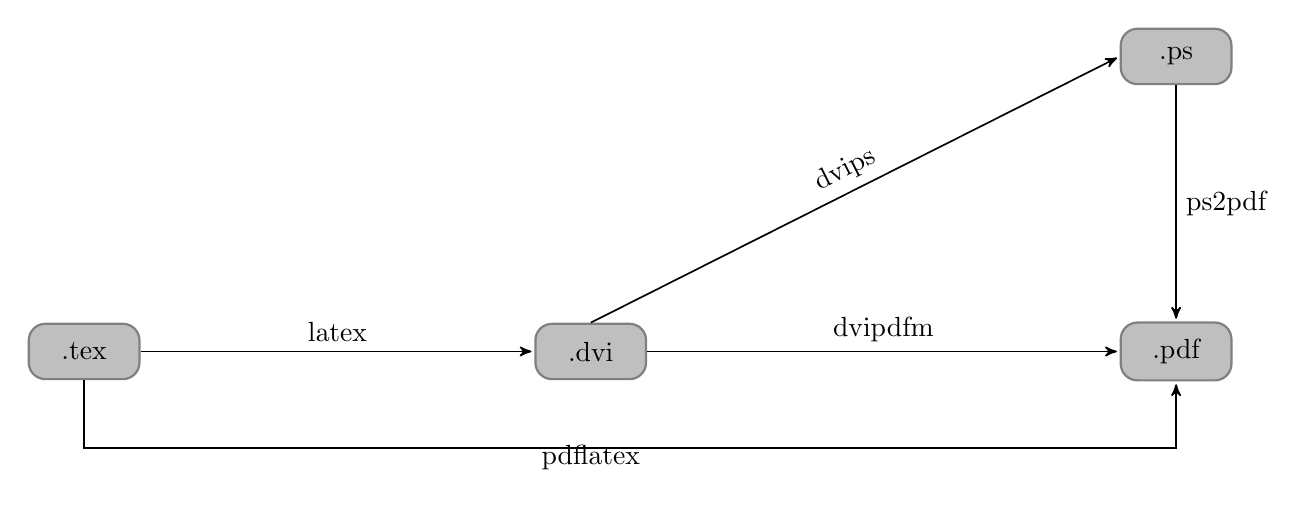
\begin{tikzpicture}
    \node[box] (tex) {.tex};
    \node[box] (dvi) [right=5 of tex] {.dvi};
    \node[box] (pdf) [right=6 of dvi] {.pdf};
    \node[box] (ps) [above=3 of pdf] {.ps};
    \path (tex) edge [arrow] node[auto] {latex} (dvi)
        (dvi) edge [arrow] node[auto] {dvipdfm} (pdf)
        (dvi.north) [arrow,draw] to node[above,sloped] {dvips} (ps.west)
        (ps) edge [arrow] node[right] {ps2pdf} (pdf)
        (tex) edge [arrow,bloop] (pdf);
    \node [below=.7 of dvi] {pdflatex};
\end{tikzpicture}
\caption{格式转换}
\label{fig:convert_format}
\end{figure}

最早的~driver~是~\verb|dvips|,它把~DVI~转换为~PS。\verb|dvipdf|~把~DVI~转为~PDF,它后来被~\verb|dvipdfm|~所取代;\verb|dvipdfm|~主要用于处理单字节字符,1999~年之后停止开发;在~\verb|dvipdfm|~基础上发展来的~\verb|dvipdfmx|~可以处理多字节编码(字符编码详见\ref{sec:encoding}节)。

pdf\TeX~是一种特殊的driver,它跳过~DVI,直接用~\TeX~源文件生成~PDF。基于~pdf\TeX~的~pdf\LaTeX~则把\LaTeX~源文件转为~PDF。

包老师倾向于~\verb|dvipdfmx|,因为它对图形格式的兼容性较好,而且擅长处理中文。

得到~DVI~后,我们可以在控制台用以下命令把它转为~PDF。
\begin{code}
dvipdfm hello_world(.dvi)
\end{code}

我们也可以把它转为~PS,接着用~Ghostscript~的一个命令行程序把它转换为~PDF,注意第二个命令需要~\verb|.ps|~后缀。一般情况下不推荐这种方法,因为它多了个步骤。
\begin{code}
dvips hello_world(.dvi)
ps2pdf hello_world.ps
\end{code}

pdf\LaTeX~用法如下。
\begin{code}
pdflatex hello_world(.tex)
\end{code}

\section{\LaTeX~语句}
\LaTeX~源文件的每一行称作一条语句(statement),语句可以分三种:命令(command)、数据(data)和注释(comment)。

命令分为两种:普通命令和环境(environment)。普通命令以\verb|\|~起始,大多只有一行;而环境包含一对起始声明和结尾声明,用于多行的场合。命令和环境可以互相嵌套。

数据就是普通内容。注释语句以~\verb|%|~起始,它在编译过程中被忽略。

例如在\ref{sec:hello_world}节例1中,第一行是注释,第二行是普通命令;第三、五行是环境的起始和结尾声明;第四行是数据。

\section{文档结构}
\subsection{文档类、序言、正文}
\LaTeX~源文件的结构分三大部分,依次为:文档类声明、序言(可选)、正文。

文档类声明用来指定文档的类型;序言(preamble)用来完成一些特殊任务,比如引入宏包,定义命令,设置环境等;文档的实际内容则放在正文部分。这里的正文指得是\verb|\begin{document}|和\verb|\end|~\verb|{document}|之间的部分,和通常人们心目中的“正文”概念有所出入。

这三部分的基本语法如下:
\begin{code}
\documentclass[options]{class}  %文档类声明
\usepackage[options]{package}   %引入宏包
...
\begin{document}                %正文
...
\end{document}
\end{code}

常用的文档类(documentclass)有三种:\verb|article、report、book|,它们的常用选项见\fref{tab:class_options}。

\begin{table}[htbp]
\centering
\caption{文档类常用选项}
\label{tab:class_options}
\begin{tabularx}{350pt}{lX}
    \toprule
    10pt, 11pt, 12pt & 正文字号,缺省10pt。\LaTeX~会根据正文字号选择标题、上下标等的字号。\\
    letterpaper, a4paper & 纸张尺寸,缺省是~letter。\\
    notitlepage, titlepage & 标题后是否另起新页。article~缺省~notitlepage,report~和~book~缺省有~titlepage。\\
    onecolumn, twocolumn & 栏数,缺省单栏。\\
    oneside, twoside & 单面双面。article~和~report~缺省单面,book~缺省双面。\\
    landscape & 打印方向横向,缺省纵向。\\
    openany, openright & 此选项只用于~report~和~book。report~缺省~openany~,book~缺省~openright。\\
    draft & 草稿模式。有时某些行排得过满,draft~模式可以在它们右边标上粗黑线提醒用户。\\
    \bottomrule
\end{tabularx}
\end{table}

\LaTeX~的核心只提供基本的功能,系统以宏包(package)的形式提供附加功能或增强原有功能。其它一些编程语言也有类似的模块化机制,比如~C/C++~的~\verb|#include|,Java~的~\verb|import|。

\subsection{标题、摘要、章节}


一份文档正文部分的开头通常有标题、作者、摘要等信息,之后是章节等层次结构,内容则散布于层次结构之间。

标题、作者、日期等命令如下,注意\verb|\maketitle|~命令要放在最后。
\begin{code}
\title{标题}
\author{作者}
\today
\maketitle
\end{code}

摘要环境用法如下:
\begin{code}
\begin{abstract}
...
\end{abstract}
\end{code}

常用的层次结构命令如下,
\begin{code}
\chapter{...}
\section{...}
\subsection{...}
\subsubsection{...}
\end{code}

每个高级层次可以包含若干低级层次。\verb|article|~中没有~\verb|chapter|,而~\verb|report|~和~\verb|book|~则支持上面所有层次。

\subsection{目录}

我们可以用~\verb|\tableofcontents|~命令来生成整个文档的目录,\LaTeX~会自动设定目录包含的章节层次,也可以用~\verb|\setcounter|~命令来指定目录层次深度。
\begin{code}
\tableofcontents
\setcounter{tocdepth}{2}
\end{code}

如果不想让某个章节标题出现在目录中,可以使用以下带~\verb|*|~的命令来声明章节。
\begin{code}
\chapter*{...}
\section*{...}
\subsection*{...}
\end{code}

类似地,我们也可以用以下命令生成插图和表格的目录,插图和表格功能将在后面章节中介绍。

\begin{code}
\listoffigures
\listoftables
\end{code}

当章节或图表等结构发生变化时,我们需要执行两遍编译命令以获得正确结果。\LaTeX~之所以设计成这样可能是因为当时的电脑内存容量有限。

\section{文字排版}
\subsection{字符输入}
文档中可以输入的内容大致可以分为:普通字符、控制符、特殊符号、注音符号、预定义字符串等。而这些内容有两种输入模式:文本模式(缺省)和数学模式,普通的行间(inline)数学模式用\verb|\$...\$|来表示。

\LaTeX~中有些字符(例如~\verb|# $ % ^ & _ { } ~ \|~等)被用作特殊的控制符,所以不能直接输入,多数需要在前面加个~\verb|\|。而~\verb|\|~本身则要用~\verb|\textbackslash|~命令来输入,因为~\verb|\\|~被用作了换行指令。很奇怪为什么不用~C~语言的~\verb|\n|,也许是因为~\TeX~的编程语言是~Pascal。

\begin{code}
\# \$ \% \^{} \& \_ \{ \} \~{} \textbackslash
\end{code}

\Fref{tab:symbol}~提供了一些符号的输入方法示例,完整的符号列表见~Scott Pakin的《The Comprehensive \LaTeX~ Symbol List》\citep{Pakin_2008}。

\begin{table}[htbp]
\centering
\caption{一些符号和预定义字符串}
\label{tab:symbol}
\begin{tabular}{llllll}
    \toprule
    \multicolumn{2}{c}{特殊符号} & \multicolumn{2}{c}{注音符号} & 
    \multicolumn{2}{c}{预定义字符串} \\
    \cmidrule(lr){1-2} \cmidrule(lr){3-4} \cmidrule(lr){5-6}
    \textcopyright  & \verb|\textcopyright|  & \aa & \verb|\aa| & 
        \today & \verb|\today| \\
    \textregistered & \verb|\textregistered| & \AA & \verb|\AA| & 
        \TeX & \verb|\TeX| \\
    $^\circ$C       & \verb|$^\circ$C|       & \ae & \verb|\ae| & 
        \LaTeX & \verb|\LaTeX| \\
    \textyen        & \verb|\textyen|        & \o  & \verb|\o| &
        \LaTeXe & \verb|\LaTeXe| \\
    \pounds         & \verb|\pounds|         & \"o & \verb|\"o| &
        \MF & \verb|\MF| \\
    \texteuro       & \verb|\texteuro|       & \^o & \verb|\^o| &
        \MP & \verb|\MP| \\
    \dots           & \verb|\dots|           & \~o & \verb|\~o| & \\
    \bottomrule
\end{tabular}
\end{table}

\subsection{换行、换页、断字}
通常~\LaTeX~会自动换行、换页。用户也可以用~\verb|\\|~或~\verb|\newline|~来强制换行;用~\verb|\newpage|~来强制换页。

一般情况下~\LaTeX~会尽量均匀地断字(Hyphenate),使得每一行的字间距分布整齐。但有时我们也需要显式指明断字位置,比如下例就指明~BASIC~这个词不能断开,而~blar-blar-blar~可以在-处断开。
\begin{code}
\hyphenation{BASIC blar-blar-blar}
\end{code}

\subsection{字样、字号}

\LaTeX~会自动调整正文、标题、章节、上下标、脚注等的字样\footnote{关于字样详见\ref{sec:typeface}节}、字号。我们也可以用\fref{tab:typeface_command}中的命令来设置字样;用\fref{tab:fontsize_command}中的命令来设置相对字号,比如正文字号是~10pt、11pt、12pt~时,tiny的字号就分别是~5pt、6pt、6pt。

\LaTeX~有一个特别的字样强调命令:\verb|\emph|,它在不同字样和装饰环境下有不同效果。比如周围文字是正体,它就是斜体;反之它就是正体。

\begin{table}[hbtp]
\centering
\caption{字样命令}
\label{tab:typeface_command}
\begin{tabular}{llll}
    \toprule
    \verb|\textrm{...}| & \textrm{roman} & 
    \verb|\textbf{...}| & \textbf{bold face} \\
    \verb|\textsf{...}| & \textsf{sans serif} & 
    \verb|\textit{...}| & \textit{italic} \\
    \verb|\texttt{...}| & \texttt{typewriter} & 
    \verb|\textsl{...}| & \textsl{slanted} \\
    \\
    \verb|\emph{...}|   & \emph{emphasized} & 
    \verb|\underline{...}|  & \underline{underline} \\
    \verb|\textsc{...}| & \textsc{Small Caps} & & \\
    \bottomrule
\end{tabular}
\end{table}

\begin{table}[htbp]
\centering
\caption{字号命令}
\label{tab:fontsize_command}
\begin{tabular}{llll}
    \toprule
    & \multicolumn{3}{c}{正文字号} \\
    \cmidrule(lr){2-4}
    命令 & 10pt & 11pt & 12pt \\
    \midrule
    \verb|\tiny|         & 5pt  & 6pt  & 6pt \\
    \verb|\scriptsize|   & 7pt  & 8pt  & 8pt \\
    \verb|\footnotesize| & 8pt  & 9pt  & 10pt \\
    \verb|\small|        & 9pt  & 10pt & 11pt \\
    \verb|\normalsize|   & 10pt & 11pt & 12pt \\
    \verb|\large|        & 12pt & 12pt & 14pt \\
    \verb|\Large|        & 14pt & 14pt & 17pt \\
    \verb|\LARGE|        & 17pt & 17pt & 20pt \\
    \verb|\huge|         & 20pt & 20pt & 25pt \\
    \verb|\Huge|         & 25pt & 25pt & 25pt \\
    \bottomrule
\end{tabular}
\end{table}

\section{常用命令环境}
\subsection{列表}

\LaTeX~中有三种列表环境:\verb|itemize、enumerate、description|,它们的一般用法如下:

\begin{demo}
\begin{itemize}
    \item C++
    \item Java
    \item HTML
\end{itemize}
\end{demo}

\begin{demo}
\begin{enumerate}
    \item C++
    \item Java
    \item HTML
\end{enumerate}
\end{demo}

\begin{demo}
\begin{description}
    \item{C++} 一种编程语言
    \item{Java} 另一种编程语言
    \item{HTML} 一种标记语言
\end{description}
\end{demo}

\subsection{对齐}
\LaTeX~中的段落缺省两端对齐(fully justified),我们也可以让段落居左、居右或居中对齐。

\begin{demo}
\begin{flushleft}
本段落\\
居左
\end{flushleft}
\end{demo}

\begin{demo}
\begin{flushright}
本段落\\
居右
\end{flushright}
\end{demo}

\begin{demo}
\begin{center}
本段落\\
居中
\end{center}
\end{demo}

\subsection{摘录}
\LaTeX~中有三种摘录环境:\verb|quote、quotation、verse|。\verb|quote|~两端都缩进,\verb|quotation|~在~\verb|quote|~的基础上增加了首行缩进,\verb|verse|~比~\verb|quote|~多了第二行起的缩进。

\begin{demo}
正文
\begin{quote}
引文两端都缩进。
\end{quote}
正文
\end{demo}

\begin{demo}
正文
\begin{quotation}
引文两端缩进,首行缩进。
\end{quotation}
正文
\end{demo}

\begin{demo}
正文
\begin{verse}
引文两端缩进,第二行起缩进。
\end{verse}
正文
\end{demo}

\subsection{原文照排}
一般文档中,命令和源代码通常使用等宽字样来表示,也就是原文照排。对此~\LaTeX~提供了~\verb|\verb|~命令(一般用于在正文中插入较短的命令)和~\verb|verbatim|~环境。后者有带~\verb|*|~的版本用来标明空格。

\begin{demo}
正文中插入\verb|command|
\begin{verbatim}
printf("Hello, world!");
\end{verbatim}
\begin{verbatim*}
printf("Hello, world!");
\end{verbatim*}
\end{demo}

\subsection{交叉引用}
我们常常需要引用文档中~\verb|section、subsection、figure、table|~等对象的编号,这种功能叫作交叉引用(cross referencing)。

\LaTeX~中可以用~\verb|\label{marker}|~命令来定义一个标记,标记名可以是任意字符串,但是在全文中须保持唯一。之后可以用~\verb|\ref{marker}|~命令来引用标记处章节或图表的编号,用~\verb|\pageref{marker}|~来引用标记处的页码。

\begin{demo}
被引用处\label{sec}\\
...\\
第\pageref{sec}页\ref{sec}节
\end{demo}

文档中新增交叉引用后,第一次执行~\verb|latex|~或~\verb|pdflatex|~编译命令时会得到类似下面的警告信息。因为第一次编译只会扫描出有交叉引用的地方,第二次编译才能得到正确结果。

\begin{code}
LaTeX Warning: There were undefined references.
...
LaTeX Warning: Label(s) may have changed. Rerun to get cross-
references right.
\end{code}

\subsection{脚注}
脚注(footnote)的一般用法如下:
\begin{demo}
这里是一段正文。\footnote{这里是一段脚注。}
\end{demo}

\section{长度单位}
\LaTeX~中的常用长度单位如\Fref{tab:unit}~所示。point~是个传统印刷业采用的单位,而~big point~是~Adobe~推出~PS~时新定义的单位。em~是个相对单位,比如当前字体是~11pt~时,1em~就是~11pt。
\begin{table}[htbp]
\caption{常用长度单位}
\label{tab:unit}
\centering
\begin{tabular}{llllll}
    \toprule
    in & 英寸 & pt & point, 1/72.27 in  & em & 当前字体中字母M的宽度 \\
    cm & 厘米 & bp & big point, 1/72 in & ex & 当前字体中字母x的高度 \\
    mm & 毫米 & pc & pica, 12 pt        & mu & math unit,1/18 em \\
    \bottomrule
\end{tabular}
\end{table}

\section{盒子}
\LaTeX~在排版时把每个对象(小到一个字母,大到一个段落)都视为一个矩形盒子(box),我们在~HTML~和~CSS~中也可以见到类似的模型。

\subsection{mbox~和~fbox}

\LaTeX~中最简单的盒子是~\verb|\mbox|~和~\verb|\fbox|。前者把一组对象组合起来,后者在此基础上加了个边框。
\begin{demo}
\mbox{010 6278 5001}
\fbox{010 6278 5001}
\end{demo}

\subsection{makebox~和~framebox}
稍复杂的~\verb|\makebox|~和~\verb|\framebox|~提供了宽度和对齐方式控制选项。这里用~l、r、s~分别代表居左、居右和分散对齐。
\begin{demo}
%语法:[宽度][对齐方式]{内容}
\makebox[100pt][l]{居左}
\framebox[100pt][r]{居右}
\end{demo}

\subsection{parbox~和~minipage}
大一些的对象比如整个段落可以用~\verb|\parbox|~命令和~\verb|\minipage|~环境,两者语法类似,也提供了对齐方式和宽度的选项。但是这里的对齐方式是指与周围内容的纵向关系,用~t、c、b~分别代表居顶、居中和居底对齐。

\begin{demo}
%语法:[对齐方式]{宽度}{内容}
\parbox[c]{90pt}{锦瑟无端五十弦,\\一弦一柱思华年。}李商隐
\end{demo}

细心的读者会发现~\verb|\parbox|~和~\verb|\minipage|~的选项排列顺序和~\verb|\makebox|~和~\verb~\framebox|~的不一致,可能出自不同的作者。

\bibliographystyle{unsrtnat}
\bibliography{reading}
\newpage

\chapter{数学}

\begin{quotation}
今有上禾三秉,中禾二秉,下禾一秉,实三十九斗;上禾二秉,中禾三秉,下禾一秉,实三十四斗;上禾一秉,中禾二秉,下禾三秉,实二十六斗。问上、中、下禾实一秉各几何?
\begin{gather*}
\begin{split}
    3x+2y+z &= 39 \\
    2x+3y+z &= 34 \\
    x+2y+3z &= 26 \\
\end{split}
\end{gather*}
\begin{flushright}
--- 《九章算术》
\end{flushright}
\end{quotation}

%\begin{quotation}
%邺下谚曰:博士买驴,书券三纸,未有驴字。
%\begin{flushright}
%--- 颜之推《颜氏家训·勉学》
%\end{flushright}
%\end{quotation}

为了使用~\AmS-\LaTeX~提供的数学功能,我们首先需要在文档的序言部分加载~\verb|amsmath|~宏包,其详细用法可参阅《amsmath User's Guide》\citep{AMS_2002}。更全面的数学内容排版可参阅~George Grätzer\footnote{匈牙利裔,加拿大~Manitoba~大学数学系教授。}的《More Math into \LaTeX, 4th Edition》\citep{Gratzer_2007}。
%\begin{code}
%\usepackage[options]{amsmath}
%\end{code}

\section{数学模式}
\LaTeX~中的数学模式有两种形式:inline~和~display。前者是指在正文插入行间数学公式,后者独立排列,可以有或没有编号。

行间公式用一对~\verb|$...$|~来输入,独立公式用~\verb|equation|~或~\verb|equation*|~环境来输入,有~\verb|*|~的版本不生成公式编号。

前文提到~\verb|\fbox|~命令可以给文本内容加个方框,数学模式下也有类似的命令~\verb|\boxed|。

\begin{demo}
爱因斯坦的$E=mc^2$方程
\begin{equation} 
    E=mc^2 
\end{equation}
\[ E=mc^2 \]
\[ \boxed{E=mc^2} \]
\end{demo}

\section{基本原素}
\subsection{字母}

英文字母在数学模式下可以直接输入,希腊字母则需要用\Fref{tab:greek}~中的命令输入,注意大写希腊字母的命令首字母也是大写。

\begin{table}[htbp]
\caption{希腊字母}
\label{tab:greek}
\centering
\begin{tabular}{llllllll}
    \toprule
    $\alpha$      & \verb|\alpha|      & $\theta$    & \verb|\theta|    & 
        $o$         & \verb|o|        & $\tau$     & \verb|\tau| \\
    $\beta$       & \verb|\beta|       & $\vartheta$ & \verb|\vartheta| & 
        $\pi$       & \verb|\pi|      & $\upsilon$ & \verb|\upsilon| \\
    $\gamma$      & \verb|\gamma|      & $\iota$     & \verb|\iota|     & 
        $\varpi$    & \verb|\varpi|   & $\phi$     & \verb|\phi| \\
    $\delta$      & \verb|\delta|      & $\kappa$    & \verb|\kappa|    & 
        $\rho$      & \verb|\rho|     & $\varphi$  & \verb|\varphi| \\
    $\epsilon$    & \verb|\epsilon|    & $\lambda$   & \verb|\lambda|   & 
        $\varrho$   & \verb|\varrho|  & $\chi$     & \verb|\chi| \\
    $\varepsilon$ & \verb|\varepsilon| & $\mu$       & \verb|\mu|       & 
        $\sigma$    & \verb|\sigma|   & $\psi$     & \verb|\psi| \\
    $\zeta$       & \verb|\zeta|       & $\nu$       & \verb|\nu|       & 
        $\varsigma$ & \verb|\varsigma|   & $\omega$   & \verb|\omega| \\
    $\eta$        & \verb|\eta|        & $\xi$       & \verb|\xi|       & 
        &                 &            & \\
    $\Gamma$      & \verb|\Gamma|      & $\Lambda$   & \verb|\Lambda|   & 
        $\Sigma$    & \verb|\Sigma|   & $\Psi$     & \verb|\Psi| \\
    $\Delta$      & \verb|\Delta|      & $\Xi$       & \verb|\Xi|       & 
        $\Upsilon$  & \verb|\Upsilon| & $\Omega$   & \verb|\Omega| \\
    $\Theta$      & \verb|\Theta|      & $\Pi$       & \verb|\Pi|       & 
        $\Phi$      & \verb|\Phi|     &            & \\
    \bottomrule
\end{tabular}
\end{table}

\subsection{指数、下标、根号}
指数或上标用~\verb|^|~表示,下标用~\verb|_|~表示,根号用~\verb|\sqrt|~表示。上下标如果多于一个字母或符号,需要用一对~\verb|{}|~括起来。
\begin{demo}
\[x_{ij}^2\quad \sqrt[2]{x}\]
\end{demo}

\subsection{分数}
分数用~\verb|\frac|~命令表示,它会自动调整字号,比如在行间公式中小一点,在独立公式则大一点。\verb|\dfrac|~命令把分数的字号显式设置为独立公式中的大小,\verb|\tfrac|~命令则把字号设为行间公式中的大小。
\begin{demo}
$\frac{1}{2} \dfrac{1}{2}$
\[\frac{1}{2} \tfrac{1}{2}\]
\end{demo}

\subsection{运算符}
有些小的运算符(operator)例如~\verb|+ - * /|~等可以直接输入,另一些则需要特殊命令。完整的数学符号参见~Scott Pakin~的《The Comprehensive \LaTeX~ Symbol List》\citep{Pakin_2008}。
\begin{code}
\[\pm \times \div \cdot \cap \cup \geq \leq \neq \approx \equiv\]
\end{code}

\begin{out}
\[\pm\quad \times\quad \div\quad \cdot\quad \cap\quad \cup\quad \geq\quad \leq\quad \neq\quad \approx\quad \equiv\]
\end{out}

和、积、极限、积分等大运算符用~\verb|\sum \prod \lim \int|~等表示。它们的上下标在行间公式中被压缩,以适应行高。。

\begin{code}
$\sum_{i=1}^n i \prod_{i=1}^n \lim_{x\to0}x^2 \int_a^b x^2 dx\$
\[\sum_{i=1}^n i \prod_{i=1}^n \lim_{x\to0}x^2 \int_a^b x^2 dx\]
\end{code}

\begin{out}
$\sum_{i=1}^n i\quad \prod_{i=1}^n\ \lim_{x\to0}x^2\ \int_a^b x^2\mathrm{d}x$
\[\sum_{i=1}^n i\quad \prod_{i=1}^n\ \lim_{x\to0}x^2\ \int_a^b x^2\mathrm{d}x\]
\end{out}

多重积分如果用多个~\verb|\int|~来输入的话,积分号间距过宽。正确的方法是用~\verb|\iint \iiint \iiiint \idotsint|~等命令输入。从下例中可以看出两种方法的差异。

\begin{out}
\[\iint\quad \iiint\quad \iiiint\quad \idotsint\]
\[\int\int\quad \int\int\int\quad \int\int\int\int\quad \int\dots\int\]
\end{out}

\subsection{分隔符}
各种括号用~\verb|() [] \{\} \langle\rangle|~等命令表示,注意花括号通常用来输入命令和环境的参数,所以在数学公式中它们前面要加~\verb|\|。因为~\LaTeX~中的~\verb+|和\|+~的应用过于随意,~amsamth~宏包推荐用~\verb|\lvert\rvert|~和~\verb|\lVert\rVert|~取而代之。

我们可以在上述分隔符前面加~\verb|\big \Big \bigg \Bigg|~等命令来调整大小。\LaTeX~原有的方法是在分隔符前面加~\verb|\left \right|~来自动调整大小,但是效果不佳,所以~amsmath~不推荐用这种方法。

\begin{out}
\[\Bigg(\bigg(\Big(\big((x+y)\big)\Big)\bigg)\Bigg)\quad 
\Bigg[\bigg[\Big[\big[[x+y]\big]\Big]\bigg]\Bigg]\quad 
\Bigg\{\bigg\{\Big\{\big\{\{x+y\}\big\}\Big\}\bigg\}\Bigg\}\]
\[\Bigg\langle\bigg\langle\Big\langle\big\langle\langle x+y \rangle\big\rangle\Big\rangle\bigg\rangle\Bigg\rangle\quad
\Bigg\lvert\bigg\lvert\Big\lvert\big\lvert\lvert x+y \rvert\big\rvert\Big\rvert\bigg\rvert\Bigg\rvert\quad
\Bigg\lVert\bigg\lVert\Big\lVert\big\lVert\lVert x+y \rVert\big\rVert\Big\rVert\bigg\rVert\Bigg\rVert\]
\end{out}

\subsection{箭头}
\Fref{tab:arrow}~列出了部分箭头的输入方法。另外还有两个命令生成的箭头可以根据上下标自动调整长度。

\begin{table}[htbp]
\caption{箭头}
\label{tab:arrow}
\centering
\begin{tabular}{llll}
    \toprule
    $\leftarrow$       & \verb|\leftarrow|      & $\longleftarrow$       & \verb|\longleftarrow| \\
    $\rightarrow$      & \verb|\rightarrow|     & $\longrightarrow$      & \verb|\longrightarrow| \\
    $\leftrightarrow$  & \verb|\leftrightarrow| & $\longleftrightarrow$  & \verb|\longleftrightarrow| \\
    $\Leftarrow$       & \verb|\Leftarrow|      & $\Longleftarrow$       & \verb|\Longleftarrow| \\
    $\Rightarrow$      & \verb|\Rightarrow|     & $\Longrightarrow$      & \verb|\Longrightarrow| \\
    $\Leftrightarrow$  & \verb|\Leftrightarrow| & $\Longleftrightarrow$  & \verb|\Longleftrightarrow| \\
    \bottomrule
\end{tabular}
\end{table}

\begin{demo}
\[\xleftarrow{x+y+z}\quad
\xrightarrow[x<y]{a*b*c}\]
\end{demo}

\subsection{标注}
\Fref{tab:accent}~列出一些短的注音符号(accent),\Fref{tab:notation}~则列出一些长的标注符号。

\begin{table}[htbp]
\caption{数学注音符号}
\label{tab:accent}
\centering
\begin{tabular}{llllllll}
    \toprule
    $\acute{x}$ & \verb|\acute{x}| & $\tilde{x}$   & \verb|\tilde{x}|   & $\mathring{x}$   & \verb|\mathring{x}|  \\
    $\grave{x}$ & \verb|\grave{x}| & $\breve{x}$ & \verb|\breve{x}| & $\dot{x}$   & \verb|\dot{x}|    \\
    $\bar{x}$  & \verb|\bar{x}|  & $\check{x}$ & \verb|\check{x}| & $\ddot{x}$  & \verb|\ddot{x}|  \\
    $\vec{x}$ & \verb|\vec{x}| & $\hat{x}$   & \verb|\hat{x}|   & $\dddot{x}$ & \verb|\dddot{x}| \\
    \bottomrule
\end{tabular}
\end{table}

\begin{table}[htbp]
\caption{长标注符号}
\label{tab:notation}
\centering
\begin{tabular}{llll}
    \toprule
    $\overline{xxx}$        & \verb|\overline{xxx}|        & $\overleftrightarrow{xxx}$  & \verb|\overleftrightarrow{xxx}| \\
    $\underline{xxx}$       & \verb|\underline{xxx}|       & $\underleftrightarrow{xxx}$ & \verb|\underleftrightarrow{xxx}| \\
    $\overleftarrow{xxx}$   & \verb|\overleftarrow{xxx}|   & $\overbrace{xxx}$           & \verb|\overbrace{xxx}| \\
    $\underleftarrow{xxx}$  & \verb|\underleftarrow{xxx}|  & $\underbrace{xxx}$          & \verb|\underbrace{xxx}| \\
    $\overrightarrow{xxx}$  & \verb|\overrightarrow{xxx}|  & $\widetilde{xxx}$           & \verb|\widetilde{xxx}| \\
    $\underrightarrow{xxx}$ & \verb|\underrightarrow{xxx}| & $\widehat{xxx}$             & \verb|\widehat{xxx}| \\
    \bottomrule
\end{tabular}
\end{table}

\subsection{省略号}
省略号用~\verb|\dots \cdots \vdots \ddots|~等命令表示,注意~\verb|\cdots|~和~\verb|\dots|~的差别。
\begin{out}
\[\dots\quad \cdots\quad \vdots\quad \ddots\]
\end{out}

\subsection{空白间距}
在数学模式中,我们可以用\Fref{tab:quad}中的命令生成不同的间距,注意负间距命令~\verb|\!|~可以用来减小间距。

\begin{table}[htbp]
\caption{空白间距}
\label{tab:quad}
\centering
\begin{tabular}{llll}
    \toprule
    \verb|\,| & 3/18 em & \verb|\quad|  & 1 em \\    
    \verb|\:| & 4/18 em & \verb|\qquad| & 2 em \\    
    \verb|\;| & 5/18 em & \verb|\!|     & -3/18 em \\
    \bottomrule
\end{tabular}
\end{table}

\section{矩阵和行列式}
数学模式下可以用~\verb|array|~环境来生成行列表。参数~\verb|{ccc}|~用于设置每列的对齐方式,\verb|l、c、r|~分别表示左中右;\verb|\\|~和~\verb|&|~用来分隔行和列。

\begin{demo}
\[\begin{array}{ccc}
x_1 & x_2 & \dots \\
x_3 & x_4 & \dots \\
\vdots & \vdots & \ddots \\
\end{array}\]
\end{demo}

\verb|amsmath|~有几个类似的环境:\verb|pmatrix、bmatrix、Bmatrix、vmatrix|~和~
\verb|Vmatrix|,它们和~\verb|array|~的主要区别是会在表两端加上~$()\; []\; \{\}\; ||\; \|\|$~等分隔符,其次这些环境没有列对齐方式参数。

行间公式可以用~\verb|smallmatrix|~环境来生成排列紧密的小矩阵。

\section{多行公式}
有时一个公式太长一行放不下,或几个公式需要写成一组,这时我们就要用到~\verb|amsmath|~提供的几个适合多行公式的环境。

\subsection{长公式}
对于多行不需要对齐的长公式,我们可以用~\verb|multline|~环境。
\begin{demo}
\begin{multline}
x=a+b+c+\\
d+e+f+g
\end{multline}
\end{demo}

需要对齐的长公式可以用~\verb|split|~环境,它本身不能单独使用,因此也称作次环境,必须包含在~\verb|equation|~或其它数学环境内。\verb|split|~环境用~\verb|\\|~和~\verb|&|~来分行和设置对齐位置。
\begin{demo}
\[ \begin{split}
x=&a+b+c+\\
  &d+e+f+g
\end{split} \]
\end{demo}

\subsection{公式组}
不需要对齐的公式组用~\verb|gather|环境,需要对齐的用~\verb|align|。
\begin{demo}
\begin{gather}
a=b+c+d\\
x=y+z
\end{gather}
\end{demo}

\begin{demo}
\begin{align}
a&=b+c+d\\
x&=y+z
\end{align}
\end{demo}

\verb|multline、gather、align|~等环境都有带~\verb|*|~的版本,它们不生成公式编号。

有多种条件的公式组用~\verb|cases|~次环境。
\begin{demo}
\[ y=\begin{cases}
-x & x<0\\
x & x\geq0
\end{cases} \]
\end{demo}

\section{定理和证明}
\LaTeX~提供了一个~\verb|\newtheorem|~命令来定义定理之类的环境,其语法如下。
\begin{code}
\newtheorem{环境名}[编号延续]{显示名}[编号层次]
\end{code}

在下例中,我们定义了四个环境:定义、定理、引理和推论,它们都在一个~\verb|section|~内编号,而引理和推论会延续定理的编号。
\begin{code}
\newtheorem{defination}{定义}[section]
\newtheorem{theorem}{定理}[section]
\newtheorem{lemma}[theorem]{引理}
\newtheorem{corollary}[theorem]{推论}
\end{code}

\newtheorem{defination}{定义}[section]
\newtheorem{theorem}{定理}[section]
\newtheorem{lemma}[theorem]{引理}
\newtheorem{corollary}[theorem]{推论}

定义了上述环境之后,我们就可以象下面这样使用它们。
\begin{demo}
\begin{defination}
Java是一种跨平台的编程语言。
\end{defination}
\end{demo}

\begin{demo}
\begin{theorem}
咖啡因会使人的大脑兴奋。
\end{theorem}
\end{demo}

\begin{demo}
\begin{lemma}
茶和咖啡都会使人兴奋。
\end{lemma}
\end{demo}

\begin{demo}
\begin{corollary}
晚上喝咖啡会导致失眠。
\end{corollary}
\end{demo}

\verb|proof|环境可以用来输入下面这样的证明,它会在证明结尾输入一个~QED~符号\footnote{拉丁语~quod erat demonstrandum~的缩写。}。

\begin{demo}
\begin{proof}[命题``物质无限可分''的证明]
一尺之棰,日取其半,万世不竭。
\end{proof}
\end{demo}

\section{数学字体}
和文本模式类似,数学模式下可以用\Fref{tab:math_font}~中的命令选择不同字体,其中有些字体需要加载~\verb|amsfonts|~宏包。

\begin{table}[htbp]
\caption{数学字体}
\label{tab:math_font}
\centering
\begin{tabular}{ccccccc}
    \toprule
    缺省 & \verb|\mathbf| & \verb|\mathit| & \verb|\mathsf| & 
        \verb|\mathcal| & \verb|\mathbb| \\
    XNZRC & $\mathbf{XNZRC}$ & $\mathit{XNZRC}$ & $\mathsf{XNZRC}$ & 
        $\mathcal{XNZRC}$ & $\mathbb{XNZRC}$ \\
    \bottomrule
\end{tabular}
\end{table}

\bibliographystyle{unsrtnat}
\bibliography{reading}
\newpage

\chapter{插图}
\label{sec:graphics}

\begin{quotation}
A picture says more than a thousand words.
\begin{flushright}
--- Shakespeare
\end{flushright}
\end{quotation}

当年~Knuth~开发~\TeX~时,GIF、JPEG、PNG、EPS~等图形格式还没有问世,所以~DVI~不能直接支持这些格式。但是高手就是高手,Knuth~在~\TeX~上留了一个后门:\verb|\special|~命令,让后面的~Driver~决定怎样处理图形。

这和当年老毛把港澳台,老邓把钓鱼岛都“留给后人解决”有异曲同工之妙。曾经有位出版社的编辑看上了包老师写的一个程序,要包老师改改当作教学辅助软件出版,但是包老师手头没有~DOS~中断的资料没办法加鼠标操作。该编辑说:你把鼠标驱动打包在软件里,让用户自己琢磨是怎么回事。

下面我们会在~\ref{sec:graphics_format}~节介绍一下~\LaTeX~所用图形格式,\ref{sec:includegraphics}~节介绍怎样插入已有的图形,\ref{sec:mp}--\ref{sec:pgf}~节讨论怎样制作矢量图形。

\section{图形格式}
\label{sec:graphics_format}

\LaTeX~支持点阵图形格式~JPEG~和~PNG,也支持矢量格式~EPS~和~PDF。对于示意图,我们应该首选矢量格式;包含大量自然色彩的图像(比如照片)应该选~JPEG,人工点阵图像应该选~PNG。

\subsection{EPS}
80~年代中后期,PS~风头之劲一时无两,人们自然会考虑把它作为文档中嵌入图形的标准格式。然而~PS~实在太强大,人们担心嵌入文档的~PS~会搞破坏,于是就产生了戴着手铐的~Encapsulated PostScript(EPS)。出于同样的原因,人们也担心嵌入~HTML~的~ActiveX、Java Applet、JavaScript~中混入恶意代码,所以才会对它们也有所限制。

早年间~DVI~经常被转换为~PS,所以~EPS~就成了~\LaTeX~的标准图形格式。

\subsection{Driver~们的口味}

\subsubsection{dvips}
\verb|dvips|~喜欢~PS,所以就爱屋及乌只支持嵌入~EPS。MiKTeX~看不惯这种垄断行为,就把~\verb|dvips|~破解,添加了对~JPEG~和~PNG~的支持。如果你反对这种黑客破解行径,只好找软件把其它图形格式转换为~EPS。

\subsubsection{pdf\LaTeX}
pdf\LaTeX~支持~JPEG、PNG和PDF,不支持~EPS。传说pdf\LaTeX~不支持~EPS~的原因是~PS~解释器的版权问题。包老师认为这种说法不可信,因为~1997~年~Hàn The Thành~发布~pdf\TeX~时~PS~已经被~PDF~赶超,Adobe~与其保护~PS~还不如保护~PDF。

\LaTeX~有两个宏包~\verb|epstopdf|~和~\verb|pst-pdf|~可以实时地(on the fly)把~EPS~转换为~PDF\footnote{在这里on the fly是指在后台处理,用户不用操心。包老师不确定把它翻译为“实时”是否合适,因为~real time~通常被翻译为实时。对于用户无须干涉、知情的情况,有人说~user transparent,也有人说~black box,语言还真奇妙。}。然而前者有安全漏洞,后者用法繁琐,用户最好还是用其它软件事先把~EPS~转为~PDF。

\subsubsection{dvipdfm}
\verb|dvipdfm|~支持~JPEG、PNG、PDF,不支持~EPS,但是它可以实时地调用~Ghostscript~把~EPS~转为~PDF。所以从图形格式支持的角度来讲,\verb|dvipdfm|~比~\verb|dvips|~和~pdf\LaTeX~都好。

那位同学说了,你这么多废话作甚,直接告诉我们用~\verb|dvipdfm|~不就完了。然而你别忘了~\verb|dvipdfm|~需要~DVI~作为输入,不幸的是用来生成~DVI~的~\verb|latex|~对~JPEG~和~PNG~有意见。

综上所述,这些~driver~都不能把图形格式痛快地通吃,所以同学们别着急,且听包老师慢慢忽悠怎样转换和处理图形格式。

\subsection{图形格式转换}

注意把点阵图形转换为矢量图形并不能提高图形本身的质量,正所谓“garbage in, garbage out”。

\subsubsection{JPEG~和~PNG~的范围框}

作为中间格式的~DVI~不包含图形本身,它只记录图形的尺寸和文件名,因为具体的图形处理由后面的~driver~负责。DVI~中图形的尺寸来自它的范围框(bounding box),而~\verb|latex|~无法从点阵图形文件中提取这一信息,所以我们需要以某种方式把范围框信息告诉它。

一种方法是打开图形文件,记下尺寸,插入图形时加上相应的参数。

另一种方法用~\verb|ebb|~程序生成一个含范围框信息的文件。比如下例会生成~\verb|graph.bb|~文件,有了它插入图形时就不需要范围框参数。注意有时此程序算出的范围框不准,不知道是它的~bug~还是包老师的人品问题。
\begin{code}
ebb graph.jpg
\end{code}

\subsubsection{其它格式转为EPS}
有很多程序都可以把点阵图形转换为~EPS,比如~\href{http://www.imagemagick.org/}{ImageMagick},以及~\href{http://www.tex.ac.uk/cgi-bin/texfaq2html?label=dvipsgraphics}{~a2ping/sam2p、bmeps、jpeg2ps、sam2p}~等。

PS~从~Level 2~开始才支持点阵图形压缩,所以在把其它格式转为~EPS~时应尽量使用~Level 2~或~3,否则输出的~EPS~会很大。

下面是一个~ImageMagick~中~\verb|convert|~程序的例子。
\begin{code}
convert photo.jpg eps2:photo.eps
\end{code}

另外还有一种~PS~虚拟打印机的方法,优点是可以把几乎所有文件“打印”成~EPS,缺点是输出的是~PS Level 1,即使驱动程序提供了其它~Level~的选项。

\begin{enumerate}
\item 找一个~PS~打印机驱动程序。Windows~安装盘附带很多打印机驱动,其中带~PS~字样的就是~PS~驱动。包老师选的是“HP Color LaserJet 8550-PS”,Adobe~提供的~PS~驱动效果不太好。其它驱动安装过程可能稍有不同。
\item 安装时端口选“FILE”,或者后面打印时选择“Print to File”。高级选项里的~PS~选项选“Encapsulated PostScript (EPS)”。
\item 打开点阵图形文件,打印到上面的虚拟打印机,输出的文件就是~EPS,但是它没有范围框。
\item 用~GSview~打开上面生成的~EPS,不用理会没范围框的警告,Options~菜单里选上“EPS Clip”,用~File~菜单的“PS to EPS”生成含范围框的~EPS。
\end{enumerate}

\subsubsection{其它格式转为~PDF}

\LaTeX~附带的~\verb|epstopdf|~程序\footnote{这个命令行程序和上面提到的~epstopdf~宏包是两样东西。}可以把~EPS~转为~PDF。类似地我们也可以安装一个~PDF~虚拟打印机,用它来把其它图形文件转为~PDF。

\section{插入图形}
\label{sec:includegraphics}

\subsection{插入命令}
如今万事俱备,只欠插入。上回讲到哪儿来着?Yeah,~Knuth~的后门~\verb|\special|。

用低级命令~\verb|\special|~来插入图形很不爽,于是~\LaTeX~v2.09~增加了~\verb|epsf|~和~\verb|psfig|~宏包。之后~\LaTeXe~推出了更好的~\verb|graphics|~和~\verb|graphicx|~宏包,这两个宏包有个共同的命令:\verb|\includegraphics|。\verb|graphicx|~版本的语法更简单,功能更强大,所以一般推荐用它。

插入图形的具体命令如下,如果是点阵图形需要加范围框参数(左上角和右下角坐标)。

\begin{code}
\includegraphics[bb=0 0 410 307]{photo.jpg}
\end{code}

若想省略文件后缀,可在插入图形前使用两个命令。前者指定一个后缀列表,让~\LaTeX~自行查找;后者告诉~\LaTeX~未知后缀的都是~EPS。
\begin{code}
\DeclareGraphicsExtensions{.eps,.mps,.pdf,.jpg,.png}
\DeclareGraphicsRule{*}{eps}{*}{}
\end{code}

\subsection{缩放、旋转}
\Fref{tab:scale_angle}~和\Fref{tab:clip}~的选项可以用来缩放、旋转和裁剪插图。

\begin{table}[htbp]
\caption{includegraphics~命令的缩放和旋转选项}
\label{tab:scale_angle}
\centering
\begin{tabularx}{350pt}{lX}
    \toprule
    scale & 缩放比例 \\
    width & 宽度 \\
    height & 高度 \\
    totalheight & 范围框高度,旋转时它不等于高度 \\
    keepaspectratio & 如果不使用它而同时指定插图的宽度、高度,长宽比可能会失调;使用它时长宽比不变,宽度、高度都不超过指定参数 \\
    angle & 旋转角度 \\
    origin & 旋转原点 \\
    \bottomrule
\end{tabularx}
\end{table}

\begin{table}[htbp]
\caption{includegraphics~命令的裁剪选项}
\label{tab:clip}
\centering
\begin{tabularx}{350pt}{lX}
    \toprule
    viewport & 可视区域的左上角和右下角坐标。\\
    trim & 左、下、右、上四边裁剪的数值。\\
    clip & 是否真正裁剪。缺省为false,不执行裁剪,多出的部分就那样放着;设置为true时执行裁剪。似乎是多此一举。\\
    \bottomrule
\end{tabularx}
\end{table}

若想深入了解~\LaTeX~插入图形的功能,请参考~Keith Reckdahl~的《Using Imported Graphics in \LaTeX~ and pdf\LaTeX》\citep{Reckdahl_2006}(简称epslatex)。

\subsection{figure环境}
插图通常需要占据大块空白,所以在文字处理软件中用户经常需要调整插图的位置。\LaTeX~有一个~\verb|figure|~环境可以自动完成这样的任务,这种自动调整位置的环境称作浮动环境。

\begin{code}
\begin{figure}[htbp]%位置选项
\centering
\includegraphics[bb=0 0 410 307,scale=.8]{photo}
\caption{10个月大的Anna}
\label{fig:anna}
\end{figure}
\end{code}

\begin{figure}[htbp]
\centering
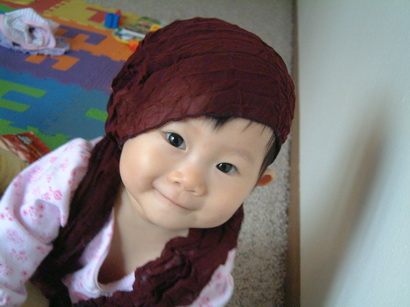
\includegraphics[bb=0 0 410 307,scale=.8]{dscf4684}
\caption{10个月大的Anna}
\label{fig:anna}
\end{figure}

上述代码中,\verb|[htbp]|~选项用来指定插图排版的理想位置,这几个字母分别代表~here、top、bottom、float page,也就是固定位置、页顶、页尾、单独的浮动页。我们可以使用这几个字母的任意组合,一般不推荐单独使用~\verb|[h]|,因为那个位置也许很不合适,\LaTeX~会很生气。

\verb|\centering|~用来使插图居中,\verb|\caption|~命令设置插图标题,\LaTeX~会自动给浮动环境的标题加上编号。注意~\verb|label|~应放在\verb|caption|~之后,否则引用时指向的是前一个插图。

\subsection{插入多幅图形}
\subsubsection{并排摆放,共享标题}
当我们需要两幅图片并排摆放,并共享标题时,可以在~\verb|figure|~环境中使用两个~\verb|\includegraphics|~命令。

\begin{fdemo}{
\centering
\includegraphics[scale=2]{examples/subfig_left.mps}
\includegraphics[scale=2]{examples/subfig_right.mps}
\captionof{figure}{反清复明}
}
\begin{figure}[htbp]
\centering
\includegraphics{left}
\includegraphics{right}
\caption{反清复明}
\end{figure}
\end{fdemo}

\subsubsection{并排摆放,各有标题}
如果想要两幅并排的图片各有自己的标题,可以在~\verb|figure|~环境中使用两个~\verb|minipage|~环境,每个环境里插入一个图。
\begin{code}
\begin{figure}[htbp]
\centering
\begin{minipage}[t]{0.3\textwidth}
    \centering
    \includegraphics{left}
    \caption{清明}
\end{minipage}
\end{code}
\begin{code}
\begin{minipage}[t]{0.3\textwidth}
    \centering
    \includegraphics{right}
    \caption{反复}
\end{minipage}
\end{figure}
\end{code}

\begin{figure}[htbp]
\centering
\begin{minipage}[t]{0.3\textwidth}
    \centering
    \includegraphics[scale=2]{examples/subfig_left.mps}
    \caption{清明}
\end{minipage}
\begin{minipage}[t]{0.3\textwidth}
    \centering
    \includegraphics[scale=2]{examples/subfig_right.mps}
    \caption{反复}
\end{minipage}
\end{figure}

\subsubsection{并排摆放,共享标题,各有子标题}
如果想要两幅并排的图片共享一个标题,并各有自己的子标题,可以使用~\verb|subfig|~宏包提供的~\verb|\subfloat|~命令。

\verb|subfloat|~命令缺少宽度参数。虽然我们可以用~\verb|\hspace|~命令调整子图的距离,子标题却只能和子图本身一样宽,就会出现折行。
\begin{code}
\usepackage{subfig}
\begin{figure}[htbp]
\centering
\subfloat[清明]{
    \label{fig:subfig_a}
    \includegraphics{left}
}
\hspace{80pt}
\subfloat[反复]{
    \label{fig:subfig_b}
    \includegraphics{right}
}
\caption{反清复明}
\end{figure}
\end{code}

每个子图可以有各自的引用,就象这个样子:\Fref{fig:subfig_a}、\Fref{fig:subfig_b}。
\begin{figure}[htbp]
\centering
\subfloat[清明]{
    \label{fig:subfig_a}
    \includegraphics[scale=2]{examples/subfig_left.mps}
}
\hspace{80pt}
\subfloat[反复]{
    \label{fig:subfig_b}
    \includegraphics[scale=2]{examples/subfig_right.mps}
}
\caption{反清复明}
\end{figure}

\subsubsection{改进的子图方法}
为了避免子标题折行,我们可以在~\verb|\subfloat|~里再嵌套个~\verb|minipage|,因为后者是有宽度的。
\begin{code}
\begin{figure}[htbp]
\centering
\subfloat[清明]{
\label{fig:improved_subfig_a}
\begin{minipage}[t]{0.3\textwidth}
    \centering
    \includegraphics{left}
\end{minipage}
}
\subfloat[反复]{
\label{fig:improved_subfig_b}
\begin{minipage}[t]{0.3\textwidth}
    \centering
    \includegraphics{right}
\end{minipage}
}
\caption{反清复明}
\end{figure}
\end{code}

\begin{figure}[htbp]
\centering
\subfloat[清明]{
\begin{minipage}[t]{0.3\textwidth}
    \centering
    \includegraphics[scale=2]{examples/subfig_left.mps}
\end{minipage}
}
\subfloat[反复]{
\begin{minipage}[t]{0.3\textwidth}
    \centering
    \includegraphics[scale=2]{examples/subfig_right.mps}
\end{minipage}
}
\caption{反清复明}
\end{figure}

\section{图形绘制工具比较}
与~\LaTeX~配套使用的绘图工具主要有三种:\MP、PSTricks~和~PGF,它们的特点如下。

\begin{itemize}
\item 工作方式。\MP~离线绘图,生成的~EPS~可以插入~\LaTeX~文档;PSTricks~和~PGF~都采用在线绘图的方式,也就是~\LaTeX~文档内直接使用绘图命令。
\item 兼容性。\MP~生成的~MPS~需要先转为~PDF~才能被~pdf\LaTeX~使用;PSTricks~生成的~EPS和~pdf\LaTeX~不兼容;PGF~提供针对各种~driver~的接口,兼容性最好。
\item 功能。PSTricks~有~PS~作后盾,功能最强;\MP~擅长处理数学内容;PGF~的流程图有独到之处。
\end{itemize}

限于篇幅,本文只对这三种工具进行简介。除了它们,用户也可以考虑一些面向~\LaTeX~的绘图前端,比如~Unix/Linux~下的~xfig~和~Windows~下的~TpX;或可以输出~EPS~的专用软件,比如~gnuplot~和~Matlab。

\section{\MP}
\label{sec:mp}

1989~年~John D. Hobby\footnote{Hobby 1985年从斯坦福获博士学位,导师就是Knuth,现供职于贝尔实验室。}开始设计一种绘图语言及其编译器,也就是~\MP。\MP~从~\MF~那里获得了大量灵感和源代码,学生从导师那里顺点东西自然是手到擒来。\MP~和~\MF~语法类似,\MP~的主要优点在于是它输出的是~EPS,而且支持彩色;\MF~输出的是点阵格式,不支持彩色。Knuth~声称自己画图时只用~\MP。

从~Hobby~主页上~\MP~的更新记录看,它的最后版本是~0.63,年份是~1994。目前~Taco Hoekwater\footnote{他也是LuaTeX开发者之一。}继续~\MP~的开发工作,最新版本是~1.005。

本文只对~\MP~作简单介绍,若想深入了解请参阅~Hobby~的《A User's Manual for MetaPost》\citep{Hobby_2007}。

\subsection{准备工作}
用户一般需要把~\MP~源文件(.mp)用一个命令行程序~\verb|mpost|~编译为一种特殊的~EPS,也称作~MPS,然后再把~MPS~插入~\LaTeX~源文件中使用。
\begin{figure}[htbp]
\centering
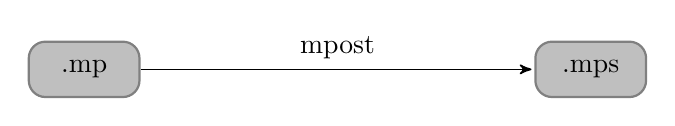
\begin{tikzpicture}
    \node[box] (mp) {.mp};
    \node[box, right=5 of mp] (mps) {.mps};
    \path (mp) edge [arrow] node[auto] {mpost} (mps);
\end{tikzpicture}
\caption{MetaPost~的编译}
\label{fig:mp}
\end{figure}

一个~\MP~源文件可以包含多个图形,一般形式如下。代码中每行语句以~\verb|;|~结尾,注释行以~\verb|%|~起始。每个图形的绘图命令包含在一对起始和结尾声明之间。文件结尾也要有一个结尾声明。
\begin{code}
beginfig(1); %图形起始
...          %绘图命令
endfig;      %图形结尾

beginfig(2);
...
endfig;
...
end;         %文件结尾
\end{code}

假如上面的源文件名字是~\verb|fig.mp|,我们可以执行以下编译命令。
\begin{code}
mpost fig(.mp)
\end{code}

编译后就会生成“fig.1、fig.2、$\cdots$”~等文件,每个文件的后缀就是相应的图形起始声明的编号。所以此编号在一个源文件中应保持唯一,否则后生成的文件就会覆盖前面的。

这样的文件名管理起来很麻烦,插入它们时也不能省略后缀,因为~\LaTeX~不能识别它们。用~\verb|\DeclareGraphicsExtensions|~来逐一声明后缀看起来很傻,自己改文件名更傻,\verb|\DeclareGraphicsRule|~也显得不够严谨。

然而~\MP~已经考虑到这个问题,为此提供了一个文件名模板命令。把下面的代码加到源文件头部,编译输出的文件名就会是“fig-01.mps、fig-02.mps、$\cdots$”。
\begin{code}
filenametemplate "%j-%2c.mps";   %加在源文件头部
\end{code}

我们也可以把这个命令加在每个图形的起始声明之前,指定个性化的输出文件名,这样可能更便于记忆。
\begin{code}
filenametemplate "flowchart.mps" %加在每个图形前面
\end{code}

MPS~可以用~GSview~查看,我们也可以用以下命令把它转为~PDF~再用~Adobe Reader~查看。

\begin{code}
epstopdf flowchart.mps
\end{code}

\subsection{基本图形对象}
为了节省空间,本节后面的示例会略去图形起始声明和结尾声明等不重要的细节。

\subsubsection{直线}

绘图命令~\verb|draw|~把几个点以直线段连接起来。\MP~中的缺省长度单位是~bp,用户也可以使用\Fref{tab:unit}~中的其它单位。我们还可以定义一个缩放系数,把坐标都转换成此系数的倍数,这样以后想缩放图形时只要改这个系数即可。

注意~\MP~中的变量赋值符号是~\verb|:=|,而~\verb|=|~用于方程式。变量在同一源文件中只须定义一次,其后的图形中都可以使用。

\begin{fdemo}{\includegraphics{examples/line.mps}}
draw (0,0)--(40,0)--(20,20)--(0,0);
u:=10pt; %缩放系数
draw (5u,0)--(9u,0)--(7u,2u)--cycle;
\end{fdemo}

几段直线或曲线可以构成一条路径(path),在路径末尾加个~\verb|cycle|~就能构成封闭路径(closed path)。上例中的两个三角形看起来都是封闭的,但是前面这个其实不是真正的封闭路径。

\subsection{点和线宽}
\verb|drawdot|~命令可以在指定坐标画一个点,为了使它醒目些我们可以换支粗一点的画笔。\MP~中的画笔缺省是直径~0.5pt~的圆形,拿它画出来的线宽就是~0.5pt。

\begin{fdemo}{\includegraphics{examples/dot.mps}}
draw (0,0)--(10u,4u);
pickup pencircle scaled 2pt;
drawdot (0,0);
drawdot (10u,4u);
\end{fdemo}

上面的~\verb|pickup|~是一种全局操作,也就是说它会影响到之后所有的绘图命令,我们也可以用~\verb|withpen|~为单个绘图命令设置画笔。

\begin{code}
draw (0,0)--(10u,4u) withpen pencircle scaled 2pt;
\end{code}

\subsubsection{曲线}
曲线和直线的命令相近,只是把连接两个点的~\verb|--|~换成了~\verb|..|。如果共用一些坐标,直线和曲线也可以混在一条语句里画。

\begin{fdemo}{\includegraphics{examples/curve.mps}}
draw (0,.5u)..(5u,3u)..(10u,1.5u)..
    (7u,0)..(5u,1.5u)..(7u,1.5u);
\end{fdemo}

\MP~的曲线用三次贝塞尔(Cubic B\'ezier)算法实现。用户可以在命令中增加~direction(方向)、Tension(张力)和~Curl(曲率)等控制,限于篇幅本文不赘述。

\subsubsection{预定义图形}
~\verb|fullcircle|~命令以原点为圆心画一个单位圆,类似的预定义图形还有~\verb|halfcircle、quartercircle、unitsquare|~等。注意单位正方形的参考点在左下而不在其中心。

通过不同的横向和纵向缩放系数,我们可以把圆形和正方形变成椭圆和长方形。

\begin{code}
draw fullcircle scaled 2u;
draw halfcircle scaled 2u shifted (3u,0);
draw quartercircle scaled 2u shifted (5u,0);
draw fullcircle xscaled 4u yscaled 2u shifted (9u,0);
draw unitsquare scaled 2u shifted (12u,-u);
draw unitsquare xscaled 4u yscaled 2u shifted (15u,-u);
\end{code}

\begin{out}
\includegraphics{examples/predefined.mps}
\end{out}

\subsection{图形控制}

\subsubsection{线型和箭头}
在绘制图形时,我们不仅可以变换线宽,也可以使用多种线型。
\begin{code}
draw (0,0)--(10u,0) dashed withdots;
draw (0,1u)--(10u,1u) dashed withdots scaled 2;
draw (0,2u)--(10u,2u) dashed evenly;
draw (0,3u)--(10u,3u) dashed evenly scaled 2;
\end{code}

\begin{out}
\includegraphics{examples/dashed.mps}
\end{out}

箭头和直线、曲线的语法相近,注意画反向箭头时需要把两个坐标用一对~\verb|()|~括起来。

\begin{fdemo}{\includegraphics{examples/arrow.mps}}
drawarrow (0,4u)--(9u,4u);
drawarrow reverse ((0,2u)--(9u,2u));
drawdblarrow (0,0)--(9u,0);
\end{fdemo}

\subsubsection{颜色和填充}
\MP~预定义的颜色有黑、白、红、绿、蓝,它们的~RGB~值分别为(0,0,0)、(1,1,1)、(1,0,0)、(0,1,0)、(0,0,1),缺省色就是黑色。

绘图命令一般都可以通过~\verb|withcolor|~参数来使用各种颜色。封闭路径可以用~\verb|fill|~命令填充。

\begin{fdemo}{\includegraphics{examples/color.mps}}
draw (0,4u)--(9u,4u) withcolor red;
draw (0,2u)--(9u,2u) withcolor green;
draw (0,0)--(9u,0) withcolor blue;
\end{fdemo}

\begin{code}
fill p scaled u;
fill p scaled u shifted (3u,0) withcolor red;
fill p scaled u shifted (6u,0) withcolor green;
fill p scaled u shifted (9u,0) withcolor blue;
\end{code}

\begin{out}
\includegraphics{examples/fill.mps}
\end{out}

另一个命令~\verb|filldraw|~可以看作是~\verb|fill+draw|,它除了填充外还会把路径用指定的画笔画一遍。然而不幸的是画边缘和填充内部只能用同一种颜色,所以它的用处不大。

除了为每个绘图命令单独指定颜色,我们也可以使用一个全局命令,使得其后的绘图命令都使用某种颜色。
\begin{code}
drawoption(withcolor blue);
\end{code}

下面的方法可以用来定义基本色以外的颜色,用基本色混色或直接用RGB值效果是一样的。

\begin{code}
color c[];
c1 := .9red + .6green + .3blue;
c2 := (.9,.6,.3);
\end{code}

\subsubsection{图形变换}
我们可以对路径进行缩放、平移、旋转等变换操作,横向和纵向缩放可以分开进行。由于旋转是围绕原点进行的,所以要注意平移和旋转的顺序。下例中定义了一个~\verb|path|~变量,以便后面重用。

\begin{code}
path p;
p := (0,0)--(2,0)--(1,1.732)--cycle;
draw p scaled u;
draw p xscaled 2u yscaled u shifted (3u,0);
draw p scaled u rotated 60 shifted (8u,0);
\end{code}

\begin{out}
\includegraphics{examples/transform.mps}
\end{out}

\subsubsection{标注}
\verb|\label|~命令可以在指定的点附近加文字标注。\MP~也可以用一对~\verb|btex|~和~\verb|etex|~来嵌入一些~\TeX~内容,比如数学标注。

\begin{code}
draw unitsquare xscaled 10u yscaled 4u;
label.top("top", (5u,4u));
label.bot("bottom", (5u,0));
label.lft("left", (0,2u));
label.rt("right", (10u,2u));
\end{code}
\begin{code}
label.ulft("upper left", (0,4u));
label.urt("upper right", (10u,4u));
label.llft("lower left", (0,0));
label.lrt("lower right", (10u,0));
label.rt(btex $E=mc^2$ etex, (3u,2u));
\end{code}

\begin{out}
\includegraphics{examples/label.mps}
\end{out}

因为用缺省方法编译生成的~MPS~不嵌入字体,当~\MP~包含文字时,GSview~就不能正常查看。这时我们可以给编译命令加个参数,生成的~MPS~就会包含字体信息。注意这种方法生成的~MPS~虽然~GSview~能查看,\verb|dvipdfmx|~却不能正常处理。

\begin{code}
mpost \prologues:=2; input fig.mp
\end{code}

\subsection{编程功能}

\subsubsection{数据类型和变量}
\MP~中有10~种基本数据类型:numeric、pair、path、pen、~color~、cmykcolor、transform、string、boolean、picture。我们已经接触过其中几种,比如缩放系数~u~就是一个~numeric,一个点的坐标是一个~pair,几个点用直线或曲线连起来是一个~path,pencircle~是一种~pen,black~是一种~color,scaled、rotated、shifted~都是~transform。

numeric~类型变量的精度是~1/65536,它的绝对值不能超过~4096,在计算过程中数值可以达到~32768。这样的规定也应归功于当年的电脑硬件,不过对于科技文档插图而言,4096~一般还是够用的。

除了缺省的~numeric,其它变量在使用之前都需要用数据类型来显式声明。相同类型的变量可以在一行语句中声明,但是带下标的变量不能放在同一行(这个规定很蹊跷)。
\begin{code}
numeric x,y,z;    %正确
numeric x1,x2,x3; %错误
numeric x[];      %正确
\end{code}

\subsubsection{数学运算}
\MP~中可以使用普通的运算符,比如~\verb|+ - * /|;也提供一些特殊的运算符,比如~\verb|a++b|~表示$\sqrt{a^2+b^2}$,\verb|a+-+b|~表示$\sqrt{a^2-b^2}$;另外\Fref{tab:math_function}~列出一些常用数学函数。

\begin{table}[htbp]
\caption{数学函数}
\label{tab:math_function}
\centering
\begin{tabular}{llll}
    \toprule
    abs     & 绝对值   & mexp & 指数 \\
    round   & 四舍五入 & mlog & 对数 \\
    ceiling & 向上圆整 & sind & 正弦 \\
    floor   & 向下圆整 & cosd & 余弦 \\
    mod     & 模余     & normaldeviate & 正态分布随机数 \\
    sqrt    & 开方     & uniformdeviate & 均匀分布随机数 \\
    \bottomrule
\end{tabular}
\end{table}

\subsubsection{循环}
当执行重复任务时,循环语句可以让程序变得简洁。注意下例中的循环语句是一条命令,之所以分成三行写是为了看起来清晰点。

\begin{fdemo}{\includegraphics{examples/loop.mps}}
draw (0,0) %注意这里没有分号
for x=1 upto 3: 
    ..(x*x,x)*u 
endfor;
\end{fdemo}

循环语句缺省步长是~1,我们也可以改用其它步长。\verb|upto|~其实就是~\verb|step 1 until|~的缩写方式。
\begin{code}
for x=1 step .5 until 3: 
\end{code}

\section{PSTricks}
\label{sec:pstricks}

PSTricks~是一个基于~PS~的宏包,有了它用户就可以直接在~\LaTeX~文档中插入绘图命令。PSTricks~早期的作者是~Timothy Van Zandt\footnote{法国Insead大学经济系教授。},初始开发年月不详,他于~1997~年退居二线,之后由~Denis Girou、Sebastian Rahtz\footnote{牛津大学计算机系网管。}、Herbert Voß~等维护。

本文只介绍~PSTricks~的基本功能,若想深入了解请参阅~Van Zandt~的《PSTricks User's Guide》\citep{Zandt_2007}。另外\Fref{tab:pst_add}~列出了一些可以和~PsTricks~配合使用的辅助宏包。

\begin{table}[htbp]
\caption{PSTricks~辅助宏包}
\label{tab:pst_add}
\centering
\begin{tabular}{llll}
    \toprule
    multido & 循环语句    & pst-eucl & 几何函数 \\    
    pst-plot & 函数绘图   & pst-math & 弧度三角函数 \\
    pst-plot3d & 三维绘图 & pstricks-add & 极坐标 \\  
    \bottomrule
\end{tabular}
\end{table}

\subsection{准备工作}
首先要引入~PSTricks~宏包。PSTricks~中缺省长度单位是~1cm,我们也可以设置自己的单位。
\psset{unit=10pt}
\begin{code}
\usepackage{pstricks}
\psset{unit=10pt}
\end{code}

绘图命令一般要放在~\verb|pspicture|~环境里,这样~\LaTeX~就会给图形预留一个矩形区域,注意这个矩形要能容纳所有图形对象。为了节省空间,在本节后面的示例代码中,~\verb|pspicture|~环境将被略去。

\begin{code}
\begin{pspicture}(0,0)(4,2)
...
\end{pspicture}
\end{code}

另外需要注意的是,嵌入~\LaTeX~的~PSTricks~生成的是~PS,\verb|dvips|~可以处理,\verb|dvipdfm|~和pdf\LaTeX~则不能。所以如果使用后两种~driver,需要先行生成~EPS。

第一种方法是把~PSTricks~代码放进一个空白的\LaTeX~页面,用它生成一个简单的~DVI。

\begin{code}
\documentclass{article}
\usepackage{pstricks}
\pagestyle{empty}   %页面样式为空

\begin{document}
\psset{unit=10pt}
\colorbox{white}{%
    \begin{pspicture}(0,0)(4,2)%
    \psdot(0,0)%
    \psdots(0,2)(2,2)(4,2)%
    \end{pspicture}%
}
\end{document}
\end{code}

然后用以下命令把~DVI~转为~EPS,\verb|-E|~参数即代表~EPS。上面代码中的~colorbox~使得生成的~EPS~有正确的范围框。

\begin{code}
dvips pst_dots(.dvi) -E -o dots.eps
\end{code}

第二种方法是用~\verb|pst-eps|~宏包,它能够在线处理~PSTricks~代码并生成~EPS,这样用户就可以在同一文件中使用该~EPS。

然而~\verb|dvipdfmx|~不能正确处理~\verb|pst-eps|~生成的~EPS。它和~\verb|\rput|、\verb|\uput|~命令,\verb|pst-plot|~宏包中的~\verb|\psaxes|~命令都不兼容。类似的~\verb|ps4pdf|~宏包和~\verb|tabularx|~宏包不兼容。

\begin{comment}
\usepackage{pst-eps}
\PSTtoEPS[bbllx=0,bblly=0,bburx=4,bbury=2,makeeps=all]
{dots.eps}{
    \psdot(0,0)
    \psdots(0,2)(2,2)(4,2)
}
\includegraphics{dots.eps}
\end{comment}

\subsection{基本图形对象}
\subsubsection{点}
我们可以用以下命令画一个或多个点。
\begin{comment}
\PSTtoEPS[bbllx=0,bblly=0,bburx=4,bbury=2,makeeps=all]
{examples/dot.eps}{
    \psdot(0,0)
    \psdots(0,2)(2,2)(4,2)
}
\end{comment}

\begin{fdemo}{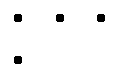
\includegraphics{examples/pst_dot.eps}}
\psdot(0,0)
\psdots(0,2)(2,2)(4,2)
\end{fdemo}

\subsubsection{直线、多边形、矩形}
\verb|\psline|~命令把多个点用直线段连接起来,线段之间的连接缺省为尖角,也可以设置圆角。
\begin{comment}
\PSTtoEPS[bbllx=0,bblly=0,bburx=9,bbury=2,makeeps=all]
{examples/line.eps}{
    \psline(0,0)(2,2)(4,0)
    \psline[linearc=.3](5,0)(7,2)(9,0)
}
\end{comment}

\begin{fdemo}{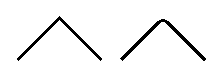
\includegraphics{examples/pst_line.eps}}
\psline(0,0)(2,2)(4,0)
\psline[linearc=.3](5,0)(7,2)(9,0)
\end{fdemo}

\verb|\pspolygon|~命令和~\verb|\psline|~类似,但是它会形成封闭路径。
\begin{comment}
\PSTtoEPS[bbllx=0,bblly=0,bburx=9,bbury=2,makeeps=all]
{examples/polygon.eps}{
    \pspolygon(0,0)(2,2)(4,0)
    \pspolygon[linearc=.3](5,0)(7,2)(9,0)
}
\end{comment}

\begin{fdemo}{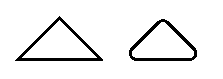
\includegraphics{examples/pst_polygon.eps}}
\pspolygon(0,0)(2,2)(4,0)
\pspolygon[linearc=.3](5,0)(7,2)(9,0)
\end{fdemo}

矩形用~\verb|\psframe|~命令,其参数就是矩形左下角和右上角的坐标。矩形也可以设置圆角。
\begin{comment}
\PSTtoEPS[bbllx=0,bblly=0,bburx=9,bbury=2,makeeps=all]
{examples/frame.eps}{
    \psframe(0,0)(4,2)
    \psframe[framearc=.3](5,0)(9,2)
}
\end{comment}

\begin{fdemo}{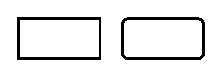
\includegraphics{examples/pst_frame.eps}}
\psframe(0,0)(4,2)
\psframe[framearc=.3](5,0)(9,2)
\end{fdemo}

\subsubsection{圆、椭圆、圆弧、扇形}
圆形用~\verb|\pscircle|~命令,参数是圆心和半径。椭圆用~\verb|\psellipse|~命令,参数是中心、长径、短径。注意这两个命令的半径参数用不同的括号,可能是作者的笔误。
\begin{comment}
\PSTtoEPS[bbllx=0,bblly=0,bburx=7,bbury=2,makeeps=all]
{examples/circle.eps}{
    \pscircle(1,1){1}
    \psellipse(5,1)(2,1)
}
\end{comment}

\begin{fdemo}{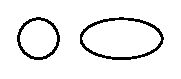
\includegraphics{examples/pst_circle.eps}}
\pscircle(1,1){1}
\psellipse(5,1)(2,1)
\end{fdemo}

圆弧用~\verb|\psarc|~命令,其参数是圆心、半径、起止角度,逆时针作图。~\verb|\psarcn|~类似,只是顺时针作图。扇形用~\verb|\pswedge|~命令。
\begin{comment}
\PSTtoEPS[bbllx=0,bblly=0,bburx=11,bbury=2,makeeps=all]
{examples/arc.eps}{
    \psarc(1,0){2}{0}{120}
    \psarcn(5,0){2}{120}{0}
    \pswedge(9,0){2}{0}{120}
}
\end{comment}

\begin{fdemo}{\includegraphics{examples/pst_arc.eps}}
\psarc(1,0){2}{0}{120}
\psarcn(5,0){2}{120}{0}
\pswedge(9,0){2}{0}{120}
\end{fdemo}

\subsubsection{曲线}
\verb|\pscurve|~命令把一系列点用平滑曲线连接起来;它的变形版本~\verb|\psecurve|~命令不显示曲线的两个端点;另一变形命令~\verb|\psccurve|~则把曲线封闭起来。

参数~\verb|showpoints=true|~用来显示曲线的构成点,此参数也可用于其它绘图命令。
\begin{comment}
\PSTtoEPS[bbllx=0,bblly=0,bburx=15,bbury=2,makeeps=all]
{examples/curve.eps}{
    \pscurve[showpoints=true](0,1)(1,2)(3,0)(4,2)(1,0)
    \psecurve[showpoints=true](5,1)(6,2)(8,0)(9,2)(5,0)
    \psccurve[showpoints=true](11,1)(12,2)(14,0)(15,2)(12,0)
}
\end{comment}

\begin{code}
\pscurve[showpoints=true](0,1)(1,2)(3,0)(4,2)(1,0)
\psecurve[showpoints=true](5,1)(6,2)(8,0)(9,2)(5,0)
\psccurve[showpoints=true](11,1)(12,2)(14,0)(15,2)(12,0)
\end{code}
\begin{out}
\includegraphics{examples/pst_curve.eps}
\end{out}

\verb|\psbezier|~命令输出一条贝塞尔曲线,其参数就是曲线的控制点。
\begin{comment}
\PSTtoEPS[bbllx=0,bblly=0,bburx=6,bbury=2,makeeps=all]
{examples/bezier.eps}{
    \psbezier[showpoints=true]
        (0,0)(2,2)(4,0)(6,2)
}
\end{comment}

\begin{fdemo}{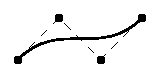
\includegraphics{examples/pst_bezier.eps}}
\psbezier[showpoints=true]
    (0,0)(2,2)(4,0)(6,2)
\end{fdemo}

抛物线用~\verb|\psparabola|~命令,它有两个参数,第一个是抛物线通过的一点,第二个是抛物线的顶点。
\begin{comment}
\PSTtoEPS[bbllx=0,bblly=0,bburx=2,bbury=2,makeeps=all]
{examples/parabola.eps}{
    \psparabola[showpoints=true]
        (2,2)(1,0)
}
\end{comment}

\begin{fdemo}{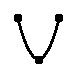
\includegraphics{examples/pst_parabola.eps}}
\psparabola[showpoints=true]
    (2,2)(1,0)
\end{fdemo}

\subsubsection{网格和坐标}
科技制图通常会用到坐标网格。\verb|\psgrid|~命令输出一个矩形网格,它有三个参数点。网格坐标标注在通过第一个点的两条直线上,第二和第三个点是矩形的两个对角顶点。当第一个参数省略时,坐标标注在通过第一个顶点的两条矩形边上。
\begin{comment}
\psset{unit=10pt}
\PSTtoEPS[bbllx=-1,bblly=-1,bburx=8.4,bbury=2.4,makeeps=all]
{examples/grid.eps}{
    \psgrid(0,0)(-1,-1)(3,2)
    \psgrid(5,0)(8,2)
}
\end{comment}

\begin{code}
\psgrid(0,0)(-1,-1)(3,2)
\psgrid(5,0)(8,2)
\end{code}
\begin{out}
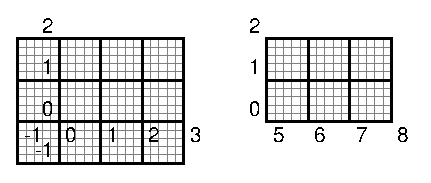
\includegraphics{examples/pst_grid.eps}
\end{out}

\verb|pst-plot|~宏包提供的~\verb|\psaxes|~命令输出坐标轴。它的参数和~\verb|\psgrid|~的类似,刻度和标注都可以灵活地设置,也可以把坐标轴改成一个矩形框的形式。
\begin{code}
\psset{unit=10pt}
\psaxes{<->}(0,0)(-1,-1)(3,2)
\psaxes[tickstyle=top,labels=none]{->}(5,0)(8,2)
\psaxes[axesstyle=frame,tickstyle=top]{->}(10,0)(13,2)
\end{code}
\begin{out}
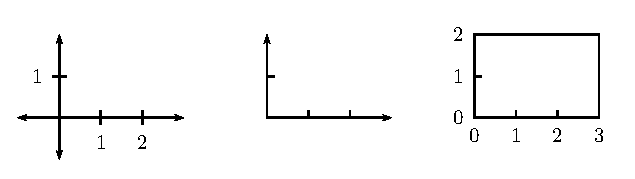
\includegraphics{examples/pst_axis.eps}
\end{out}

\subsection{图形控制}
\subsubsection{线型和箭头}
PSTricks~中的缺省线宽是~0.8pt,缺省线型是实线。以下参数可以控制单个绘图命令的线宽和线型。
\begin{comment}
\psset{unit=10pt}
\PSTtoEPS[bbllx=0,bblly=0,bburx=9,bbury=4,makeeps=all]
{examples/linestyle.eps}{
    \psline[linewidth=1.5pt](0,4)(9,4)
    \psline[linestyle=dotted](0,2)(9,2)
    \psline[linestyle=dashed](0,0)(9,0)
}
\end{comment}

\begin{fdemo}{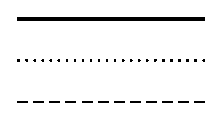
\includegraphics{examples/pst_linestyle.eps}}
\psline[linewidth=1.5pt](0,4)(9,4)
\psline[linestyle=dotted](0,2)(9,2)
\psline[linestyle=dashed](0,0)(9,0)
\end{fdemo}

我们也可以用命令~\verb|\psset|~命令来设置全局参数。
\begin{code}
\psset{linewidth=1pt,linestyle=dashed}
\end{code}

以下参数可以控制绘图命令的箭头。
\begin{comment}
\PSTtoEPS[bbllx=0,bblly=0,bburx=9,bbury=4,makeeps=all]
{examples/arrow.eps}{
    \psline{->}(0,4)(9,4)
    \psline{<-}(0,2)(9,2)
    \psline{<->}(0,0)(9,0)
}
\end{comment}

\begin{fdemo}{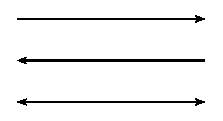
\includegraphics{examples/pst_arrow.eps}}
\psline{->}(0,4)(9,4)
\psline{<-}(0,2)(9,2)
\psline{<->}(0,0)(9,0)
\end{fdemo}

\subsubsection{颜色和填充}
PSTricks~预定义的颜色有~black、darkgray、gray、lightgray、white~等灰度颜色,也有~red、green、blue、cyan、magenta、yellow~等彩色。我们也可以自定义灰度颜色和彩色。

\begin{code}
\newgray{mygray}{.3}
\newrgbcolor{mycolor}{.3 .4 .5}
\end{code}

以下参数可以控制单个绘图命令的颜色,我们也可以用~\verb|\psset|~命令设置全局参数。
\begin{comment}
\PSTtoEPS[bbllx=0,bblly=0,bburx=9,bbury=4,makeeps=all]
{examples/color.eps}{
    \psline[linecolor=red](0,4)(9,4)
    \psline[linecolor=green](0,2)(9,2)
    \psline[linecolor=blue](0,0)(9,0)
}
\end{comment}

\begin{fdemo}{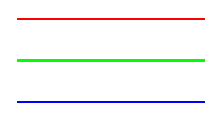
\includegraphics{examples/pst_color.eps}}
\psline[linecolor=red](0,4)(9,4)
\psline[linecolor=green](0,2)(9,2)
\psline[linecolor=blue](0,0)(9,0)
\end{fdemo}

以下参数可以控制单个绘图命令的填充模式和填充颜色,注意只有封闭路径才可以填充。
\begin{comment}
\PSTtoEPS[bbllx=0,bblly=0,bburx=11,bbury=2,makeeps=all]
{examples/fill.eps}{
    \pscircle[fillstyle=solid,fillcolor=red](1,1){1}
    \pscircle[fillstyle=vlines](4,1){1}
    \pscircle[fillstyle=hlines](7,1){1}
    \pscircle[fillstyle=crosshatch](10,1){1}
}
\end{comment}

\begin{code}
\pscircle[fillstyle=solid,fillcolor=red](1,1){1}
\pscircle[fillstyle=vlines](4,1){1}
\pscircle[fillstyle=hlines](7,1){1}
\pscircle[fillstyle=crosshatch](10,1){1}
\end{code}
\begin{out}
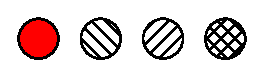
\includegraphics{examples/pst_fill.eps}
\end{out}

\subsection{对象布局}
\subsubsection{平移}
参数~\verb|origin|~可以让一个图形对象平移到指定的坐标点,我们也可以用~\verb|\psset|~命令设置全局平移参数。
\begin{comment}
\PSTtoEPS[bbllx=0,bblly=0,bburx=7,bbury=2,makeeps=all]
{examples/origin.eps}{
    \psframe(0,0)(3,2)
    \psframe[origin={4,0}](0,0)(3,2)
}
\end{comment}

\begin{fdemo}{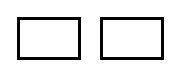
\includegraphics{examples/pst_origin.eps}}
\psframe(0,0)(3,2)
\psframe[origin={4,0}](0,0)(3,2)
\end{fdemo}

\subsubsection{旋转}
\verb|\rput|~命令可以对一个图形对象同时进行旋转和平移操作。它有两个参数,第一个是旋转角度,第二个是平移到的坐标点。
\begin{fdemo}{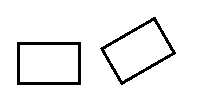
\includegraphics{examples/pst_rput.eps}}
\psframe(0,0)(3,2)
\rput{30}(5,0){\psframe(0,0)(3,2)}
\end{fdemo}

\subsubsection{文字标注}
\verb|\rput|~命令还可以在指定的坐标点标注文字,这时它的第一个参数是坐标点相对于标注的位置。其取值可以是纵向的~t、b(上下),或横向的~l、r(左右),也可以是纵向和横向位置的组合。
\begin{fdemo}{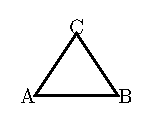
\includegraphics{examples/pst_label.eps}}
\pspolygon(0,0)(4,0)(2,3)
\rput[r](0,0){A}
\rput[l](4,0){B}
\rput[b](2,3){C}
\end{fdemo}

\verb|\rput|~生成的标注就在坐标点上,有时会感觉离图形太近。另一个命令~\verb|\uput|~则生成缺省距离指定坐标点~5pt的标注,它的第一个参数是标注相对于坐标点的角度。
\begin{fdemo}{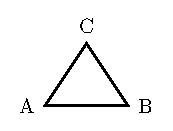
\includegraphics{examples/pst_uput.eps}}
\pspolygon(0,0)(4,0)(2,3)
\uput[l](0,0){A}
\uput[r](4,0){B}
\uput[u](2,3){C}
\end{fdemo}

\verb|\uput|~的角度参数可以是任意角度,也可以是字母,参见。注意~\verb|\uput|~的角度参数和~\verb|\rput|~命令的参考点位置参数的定义几乎正好相反,这也许反映了作者洒脱的风格。

\begin{table}[htbp]
\caption{uput~命令的角度参数}
\label{tab:uput}
\centering
\begin{tabular}{lrlr}
    \toprule
    r &   0$^\circ$ & ur &  45$^\circ$ \\
    u &  90$^\circ$ & ul & 135$^\circ$ \\
    l & 180$^\circ$ & dl & 225$^\circ$ \\
    d & 270$^\circ$ & dr & 315$^\circ$ \\
    \bottomrule
\end{tabular}
\end{table}

\section{PGF}
\label{sec:pgf}
PGF~和~Beamer~的作者都是~Till Tantau\footnote{德国Lübeck大学计算机研究所教授。}。Tantau~当初开发~Beamer~是为了应付~2003~年他的博士学位论文答辩,之后它在~CTAN~上流行开来。2005~年~PGF~从~Beamer~项目中分离出来,成为一个独立的宏包。

本文只对~PGF~作简单介绍,若想深入了解请参阅~Tantau~的《TikZ and PGF Manual》\citep{Tantau_2008}。

\subsection{准备工作}
一般人们并不直接使用~PGF~命令,而是通过它前端~TikZ~来调用~PGF。在引用~\verb|tikz|~宏包之前,用户需要设置~PGF~系统~driver。
\begin{code}
\def\pgfsysdriver{pgfsys-dvipdfmx.def}
\usepackage{tikz}
\end{code}

PGF~的缺省长度单位是~1cm,我们也可以改用其它单位。注意这样预定义的长度单位有时会失效,这可能是~PGF~的~bug。
\begin{code}
\pgfsetxvec{\pgfpoint{10pt}{0}}
\pgfsetyvec{\pgfpoint{0}{10pt}}
\end{code}

TikZ~提供一个~\verb|tikz|~命令和一个~\verb|tikzpicture|~环境,具体绘图指令可以放在~\verb|tikz|~后面,也可以放在~\verb|tikzpicture|~中间。两种方法效果相同,用户可以任意选择。为了节省空间,本节的示例将省略部分环境代码。
\begin{code}
\tikz ...   %绘图命令
\begin{tikzpicture}
...         %绘图命令
\end{tikzpicture}
\end{code}

\subsection{基本图形对象}
\subsubsection{直线、多边形、矩形}
TikZ~中直线的语法和~\MP~类似,加~\verb|cycle|~参数才能构成真正的封闭路径。
\begin{fdemo}{
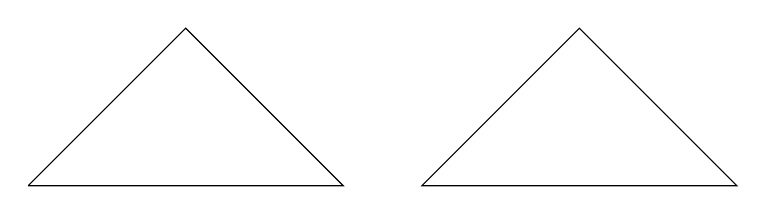
\begin{tikzpicture}
\draw (0,0)--(4,0)--(2,2)--(0,0);
\draw (5,0)--(9,0)--(7,2)--cycle;
\end{tikzpicture}
}
\draw (0,0)--(4,0)--(2,3)--(0,0);
\draw (5,0)--(9,0)--(7,3)--cycle;
\end{fdemo}

矩形命令如下,它的两个参数是矩形的两个对角顶点。
\begin{fdemo}{
\begin{tikzpicture}
\draw (0,0) rectangle (4,2);
\end{tikzpicture}
}
\draw (0,0) rectangle (4,2);
\end{fdemo}

\subsubsection{圆、椭圆、弧}
圆和椭圆命令如下,圆的参数是圆心和半径,椭圆的参数是中心、长径、短径。
\begin{fdemo}{
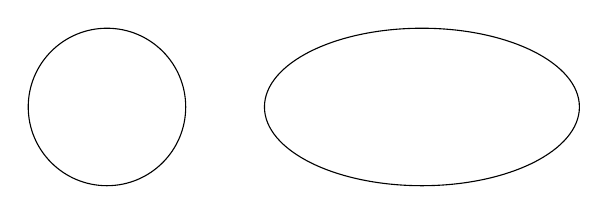
\begin{tikzpicture}
\draw (1,1) circle (1);
\draw (5,1) ellipse (2 and 1);
\end{tikzpicture}
}
\draw (1,1) circle (1);
\draw (5,1) ellipse (2 and 1);
\end{fdemo}

圆弧和椭圆弧命令如下,圆弧的参数是起始点,起始角度、终止角度、半径;椭圆弧则把半径换成了长径和短径。
\begin{fdemo}{
\begin{tikzpicture}
\draw (2,1) arc (0:270:1);
\draw (7,1) arc (0:270:2 and 1);
\end{tikzpicture}
}
\draw (2,1) arc (0:270:1);
\draw (7,1) arc (0:270:2 and 1);
\end{fdemo}

\subsubsection{曲线和抛物线}
曲线命令如下,中间的参数是控制点。
\begin{fdemo}{
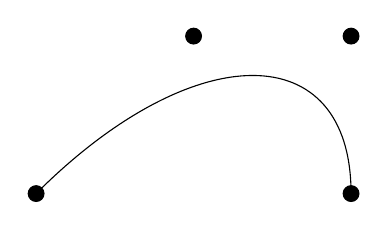
\begin{tikzpicture}
\draw (0,0) .. controls (2,2) 
    and (4,2) .. (4,0);
\filldraw (0,0) circle (.1)
    (2,2) circle (.1)
    (4,2) circle (.1)
    (4,0) circle (.1);
\end{tikzpicture}
}
\draw (0,0) .. controls (2,2) 
    and (4,2) .. (4,0);
\end{fdemo}

抛物线命令如下,除了起止点还可以指定顶点。
\begin{fdemo}{
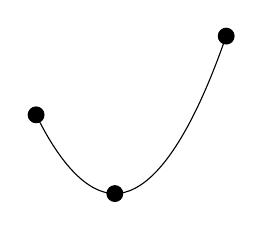
\begin{tikzpicture}
\draw (-1,1) parabola bend (0,0) (1.414,2);
\filldraw (-1,1) circle (.1)
    (0,0) circle (.1)
    (1.414,2) circle (.1);
\end{tikzpicture}
}
\draw (-1,1) parabola 
    bend (0,0) (1.414,2);
\end{fdemo}

\subsection{图形控制}
\subsubsection{线型和箭头}
绘图命令可以设置线型和箭头参数。
\begin{fdemo}{
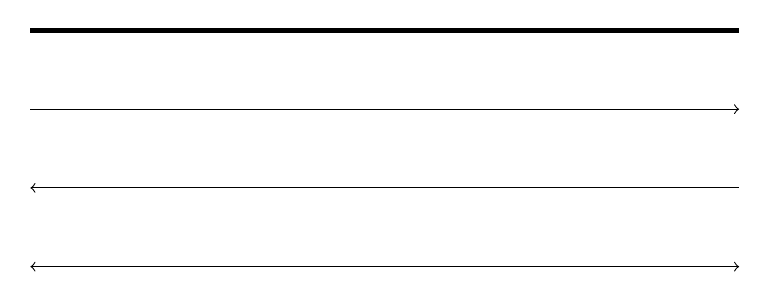
\begin{tikzpicture}
\draw[line width=2pt] (0,3)--(9,3);
\draw[->] (0,2)--(9,2);
\draw[<-] (0,1)--(9,1);
\draw[<->] (0,0)--(9,0);
\end{tikzpicture}
}
\draw[line width=2pt] (0,0)--(9,0);
\draw[->] (0,1)--(9,1);
\draw[<-] (0,2)--(9,2);
\draw[<->] (0,3)--(9,3);
\end{fdemo}

\subsubsection{颜色、填充、阴影}
颜色参数的用法如下。PGF~可以使用~\verb|xcolor|~宏包\citep{Kern_2007}中定义的所有颜色。
\begin{fdemo}{
\begin{tikzpicture}
\draw[red] (0,4)--(9,4);
\draw[green] (0,2)--(9,2);
\draw[blue] (0,0)--(9,0);
\end{tikzpicture}
}
\draw[red] (0,4)--(9,4);
\draw[green] (0,2)--(9,2);
\draw[blue] (0,0)--(9,0);
\end{fdemo}

封闭路径可以用颜色填充,\verb|\filldraw|~命令可以分别指定边框色和填充色。
\begin{fdemo}{
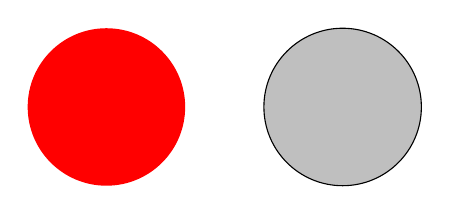
\begin{tikzpicture}
\fill[red] (1,1) circle (1);
\filldraw[fill=lightgray,draw=black] 
    (4,1) circle (1);
\end{tikzpicture}
}
\fill[red] (1,1) circle (1);
\filldraw[fill=lightgray,draw=black] 
    (4,1) circle (1);
\end{fdemo}

\verb|\shade|~命令可以产生渐变和光影效果,缺省是从上到下,灰色渐变为白色。我们也可以使用其它方向和颜色的渐变。
\begin{code}
\shade (0,0) rectangle (2,2);
\shade[left color=red,right color=orange] (3,0) rectangle (5,2);
\shade[inner color=red,outer color=orange] (6,0) rectangle (8,2);
\shade[ball color=blue] (10,1) circle (1);
\end{code}

\begin{out}
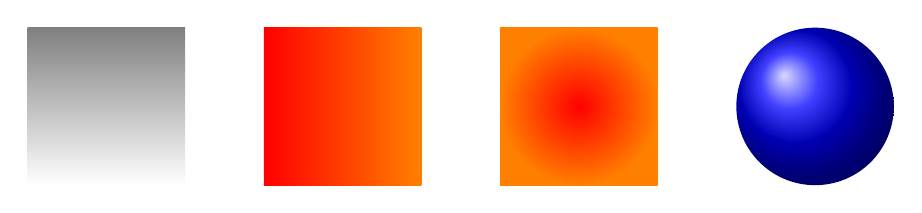
\begin{tikzpicture}
\shade (0,0) rectangle (2,2);
\shade[left color=red,right color=orange] (3,0) rectangle (5,2);
\shade[inner color=red,outer color=orange] (6,0) rectangle (8,2);
\shade[ball color=blue] (10,1) circle (1);
\end{tikzpicture}
\end{out}

\subsubsection{图形变换}
对图形对象可以进行平移和旋转操作,注意如果两种操作同时进行,它们是有顺序的。注意预定义的长度单位在这里对平移参数失效。
\begin{code}
\draw (0,0) rectangle (2,2);
\draw[xshift=30pt] (0,0) rectangle (2,2);
\draw[xshift=75pt,rotate=45] (0,0) rectangle (2,2);
\end{code}

\begin{out}
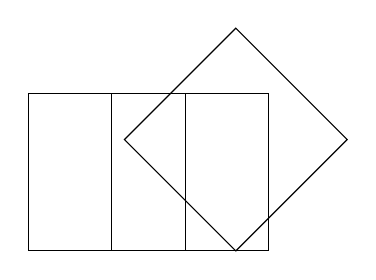
\begin{tikzpicture}
\draw (0,0) rectangle (2,2);
\draw[xshift=30pt] (0,0) rectangle (2,2);
\draw[xshift=75pt,rotate=45] (0,0) rectangle (2,2);
\end{tikzpicture}
\end{out}

\subsection{样式}
PGF~比~\MP~和~PSTricks~多了一个有趣的概念:样式(style),它的思路和~HTML~的~CSS~相近。我们可以先定义两种样式,
\tikzset{
    myline/.style={line width=2pt},
    myblueline/.style={myline,blue}
}
\begin{code}
\tikzset{
    myline/.style={line width=2pt},
    myblueline/.style={myline,blue}
}
\end{code}

然后就可以在绘图命令中这样使用样式。
\begin{fdemo}{
\begin{tikzpicture}
\draw[myline] (0,2)--(9,2);
\draw[myblueline] (0,0)--(9,0);
\end{tikzpicture}
}
\draw[myline] (0,2)--(9,2);
\draw[myblueline] (0,0)--(9,0);
\end{fdemo}

除了用~\verb|\tikzset|~命令定义样式,我们也可以在~\verb|tikzpicture|~环境头部声明样式。前者是全局性的,后者则是局部性的。
\begin{code}
\begin{tikzpicture}[
    thickline/.style=2pt,
    bluethickline/.style={thickline,color=blue}
]
...
\end{tikzpicture}
\end{code}

注意在样式中预定义长度单位有时会失效,所以最好使用绝对单位。

\subsection{流程图}
\subsubsection{节点}
PGF~中的节点(node)可以是简单的标签,也可以有各种形状的边框,还可以有各种复杂的属性。比如下例中的节点样式:\verb|box|,它的边框是矩形,有圆角;它有最小宽度、高度、文字和边框的距离,边框和填充颜色等属性。

\begin{code}
\tikzset{
    box/.style={rectangle, rounded corners=6pt, 
        minimum width=50pt, minimum height=20pt, inner sep=6pt, 
        draw=gray,thick, fill=lightgray}
}
\end{code}

除了上述类别属性,节点还可以有名字、位置等属性。在下例中,我们先画了三个有名字的文本框;然后用箭头把文本框连接起来,注意连接时要引用文本框的名字;接着在箭头上加了标签。
\begin{code}
\node[box] (tex) at(0,0) {.tex};  %文本框
\node[box] (dvi) at(10,0) {.dvi}; %文本框
\node[box] (pdf) at(20,0) {.pdf}; %文本框
\draw[->] (tex)--(dvi);           %箭头
\draw[->] (dvi)--(pdf);           %箭头
\node at (5,1) {latex};           %标签
\node at (15,1) {dvipdfmx};       %标签
\end{code}

\begin{out}
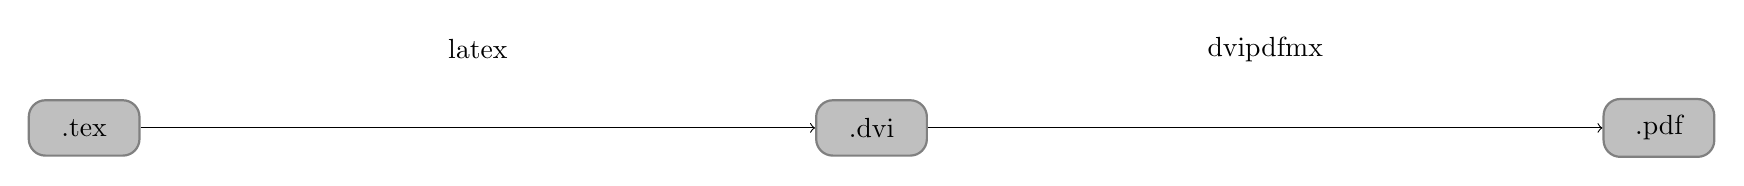
\begin{tikzpicture}
\node[box] (tex) at(0,0) {.tex};
\node[box] (dvi) at(10,0) {.dvi};
\node[box] (pdf) at(20,0) {.pdf};
\draw[->] (tex)--(dvi);
\draw[->] (dvi)--(pdf);
\node at (5,1) {latex};
\node at (15,1) {dvipdfmx};
\end{tikzpicture}
\end{out}

在上例中的节点都使用了绝对位置,PGF~中还可以使用更灵活一点的相对位置。比如在下例中,dvi~节点在~tex~节点右边~50pt~处(我们前面定义的基本长度单位是~10pt),而~pdf~节点又在~dvi~节点右边~50pt~处。

箭头可以换为专门用来连接节点的~\verb|edge|~;标签也改成相对位置,箭头上方~5pt~处。
\begin{code}
\node[box] (tex) {.tex};
\node[box,right=5 of tex] (dvi) {.dvi};
\node[box,right=6 of dvi] (pdf) {.pdf};
\path (tex) edge[->]  node[above=.5] {latex} (dvi)
    (dvi) edge[->] node[above=.5] {dvipdfmx} (pdf);
\end{code}

\begin{out}
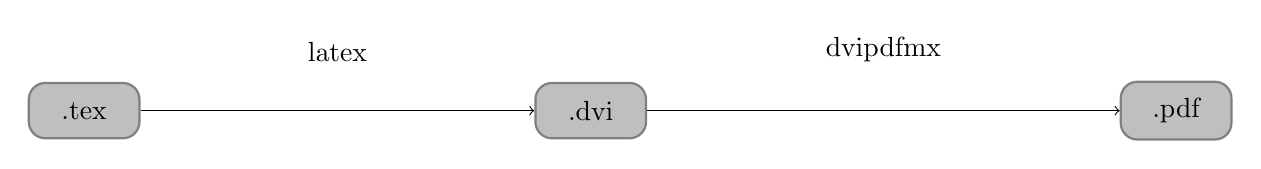
\begin{tikzpicture}
\node[box] (tex) {.tex};
\node[box,right=5 of tex] (dvi) {.dvi};
\node[box,right=6 of dvi] (pdf) {.pdf};
\path (tex) edge[->]  node[above=.5] {latex} (dvi)
    (dvi) edge[->] node[above=.5] {dvipdfmx} (pdf);
\end{tikzpicture}
\end{out}

\subsubsection{树}
下面是一棵简单的树。我们可以用一个参数控制相邻节点的距离,预定义长度单位对此参数也会失效。
\begin{code}
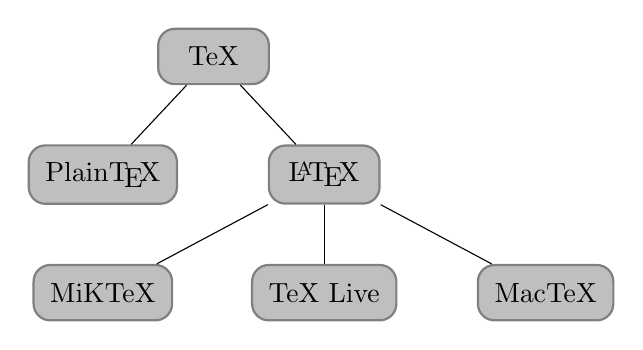
\begin{tikzpicture}[sibling distance=80pt]
\node[box] {TeX}
    child {node[box] {Plain\TeX}}
    child {node[box] {\LaTeX}
        child {node[box] {MiKTeX}}
        child {node[box] {TeX Live}}
        child {node[box] {MacTeX}}
    };
\end{tikzpicture}
\end{code}

\begin{out}
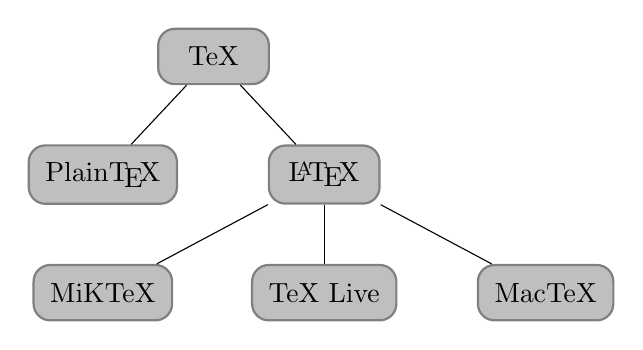
\begin{tikzpicture}[sibling distance=80pt]
\node[box] {TeX}
    child {node[box] {Plain\TeX}}
    child {node[box] {\LaTeX}
        child {node[box] {MiKTeX}}
        child {node[box] {TeX Live}}
        child {node[box] {MacTeX}}
    };
\end{tikzpicture}
\end{out}

\bibliographystyle{unsrtnat}
\bibliography{reading}
\newpage

\chapter{表格}
\label{sec:tables}

\section{简单表格}
\verb|tabular|~环境提供了最简单的表格功能。它用~\verb|\hline|~命令代表横线,\verb+|+~代表竖线,用~\verb|&|~来分栏。每个栏位的对齐方式可以用~l、c、r(左中右)来控制。
\begin{code}
\begin{tabular}{|l|c|r|}
    \hline 
    操作系统 & 发行版 & 编辑器 \\
    \hline 
    Windows & MikTeX & TeXnicCenter \\
    \hline 
    Unix/Linux & TeX Live & Emacs \\
    \hline 
    Mac OS & MacTeX & TeXShop \\
    \hline 
\end{tabular}
\end{code}

\begin{tabular}{|l|c|r|}
    \hline 
    操作系统 & 发行版 & 编辑器 \\
    \hline 
    Windows & MikTeX & TeXnicCenter \\
    \hline 
    Unix/Linux & TeX Live & Emacs \\
    \hline 
    Mac OS & MacTeX & TeXShop \\
    \hline 
\end{tabular}
\ \\

和针对插图的~\verb|figure|~环境类似,\LaTeX~还有另一个针对表格的浮动环境~\verb|table|。我们可以用它给上面的示例穿件马甲,顺便把表格简化为科技文献中常用的三线表。

\begin{code}
\begin{table}[htbp]
\caption{浮动环境中的三线表}
\label{tab:threesome}
\centering
\begin{tabular}{lll}
    \hline 
    操作系统 & 发行版 & 编辑器 \\
    \hline 
    Windows & MikTeX & TeXnicCenter \\
    Unix/Linux & TeX Live & Emacs \\
    Mac OS & MacTeX & TeXShop \\
    \hline 
\end{tabular}
\end{table}
\end{code}

\begin{table}[htbp]
\caption{浮动环境中的三线表}
\label{tab:threesome}
\centering
\begin{tabular}{lll}
    \hline 
    操作系统 & 发行版 & 编辑器 \\
    \hline 
    Windows & MikTeX & TeXnicCenter \\
    Unix/Linux & TeX Live & Emacs \\
    Mac OS & MacTeX & TeXShop \\
    \hline 
\end{tabular}
\end{table}

完美主义者可能觉得上面示例中的三条线一样粗不够美观,这时可以使用~\verb|booktabs|~宏包\citep{Fear_2005}的几个命令。

\begin{code}
\begin{table}[htbp]
\caption{浮动环境中的三线表}
\centering
\begin{tabular}{lll}
    \toprule
    操作系统 & 发行版 & 编辑器 \\
    \midrule
    Windows & MikTeX & TeXnicCenter \\
    Unix/Linux & TeX Live & Emacs \\
\end{code}

\begin{code}
    Mac OS & MacTeX & TeXShop \\
    \bottomrule
\end{tabular}
\end{table}
\end{code}

\begin{table}[htbp]
\caption{\texttt{booktabs}~宏包的效果}
\centering
\begin{tabular}{lll}
    \toprule
    操作系统 & 发行版 & 编辑器 \\
    \midrule
    Windows & MikTeX & TeXnicCenter \\
    Unix/Linux & TeX Live & Emacs \\
    Mac OS & MacTeX & TeXShop \\
    \bottomrule
\end{tabular}
\end{table}

\section{表格宽度}
有时我们需要控制某栏位宽度,可以将其对齐方式参数从~\verb|l、c、r|~改为~\verb|p{宽度}|~。
\begin{code}
\begin{table}[htbp]
\caption{控制栏位宽度}
\centering
\begin{tabular}{p{100pt}p{100pt}p{100pt}}
    \toprule
    操作系统 & 发行版 & 编辑器 \\
    \midrule
    Windows & MikTeX & TeXnicCenter \\
    Unix/Linux & TeX Live & Emacs \\
    Mac OS & MacTeX & TeXShop \\
    \bottomrule
\end{tabular}
\end{table}
\end{code}

\begin{table}[htbp]
\caption{控制栏位宽度}
\centering
\begin{tabular}{p{100pt}p{100pt}p{100pt}}
    \toprule
    操作系统 & 发行版 & 编辑器 \\
    \midrule
    Windows & MikTeX & TeXnicCenter \\
    Unix/Linux & TeX Live & Emacs \\
    Mac OS & MacTeX & TeXShop \\
    \bottomrule
\end{tabular}
\end{table}

若想控制整个表格的宽度可以使用~\verb|tabularx|~宏包,\verb|X|~参数表示某栏可以折行。

\begin{code}
\begin{table}[htbp]
\caption{控制表格宽度}
\centering
\begin{tabularx}{350pt}{lXlX}
    \toprule
    李白 & 平林漠漠烟如织,寒山一带伤心碧。暝色入高楼,有人楼上愁。玉梯空伫立,宿鸟归飞急。何处是归程,长亭更短亭。& 
    泰戈尔 & 夏天的飞鸟,飞到我的窗前唱歌,又飞去了。秋天的黄叶,它们没有什么可唱,只叹息一声,飞落在那里。\\
    \bottomrule
\end{tabularx}
\end{table}
\end{code}

\begin{table}[htbp]
\caption{控制表格宽度}
\centering
\begin{tabularx}{350pt}{lXlX}
    \toprule
    李白 & 平林漠漠烟如织,寒山一带伤心碧。暝色入高楼,有人楼上愁。玉阶空伫立,宿鸟归飞急。何处是归程,长亭更短亭。& 
    泰戈尔 & 夏天的飞鸟,飞到我的窗前唱歌,又飞去了。秋天的黄叶,它们没有什么可唱,只叹息一声,飞落在那里。\\
    \bottomrule
\end{tabularx}
\end{table}

\section{跨行、跨列表格}
有时某栏需要横跨几列,我们可以使用~\verb|\multicolumn|~命令。它的前两个参数指定横跨列数和对齐方式。\verb|booktabs|~宏包的~\verb|\cmidrule|~命令用于横跨几列的横线。
\begin{code}
\begin{table}[htbp]
\caption{跨栏表格}
\centering
\begin{tabular}{lll}
    \toprule
    & \multicolumn{2}{c}{常用工具} \\
    \cmidrule{2-3}
    操作系统 & 发行版 & 编辑器 \\
    \midrule
    Windows & MikTeX & TeXnicCenter \\
    Unix/Linux & TeX Live & Emacs \\
    Mac OS & MacTeX & TeXShop \\
    \bottomrule
\end{tabular}
\end{table}
\end{code}

\begin{table}[htbp]
\caption{跨栏表格}
\centering
\begin{tabular}{lll}
    \toprule
    & \multicolumn{2}{c}{常用工具} \\
    \cmidrule{2-3}
    操作系统 & 发行版 & 编辑器 \\
    \midrule
    Windows & MikTeX & TeXnicCenter \\
    Unix/Linux & TeX Live & Emacs \\
    Mac OS & MacTeX & TeXShop \\
    \bottomrule
\end{tabular}
\end{table}

跨行表格需要使用~\verb|multirow|~宏包,\verb|\multirow|~命令的前两个参数是竖跨的行数和宽度。
\begin{code}
\usepackage{multirow}
...
\begin{table}[htbp]
\caption{跨行表格}
\centering
\begin{tabular}{lllc}
\end{code}
\begin{code}
    \toprule
    操作系统 & 发行版 & 编辑器 & 用户体验\\
    \midrule
    Windows & MikTeX & TeXnicCenter & 
    \multirow{3}{*}{\centering 爽} \\
    Unix/Linux & TeX Live & Emacs \\
    Mac OS & MacTeX & TeXShop \\
    \bottomrule
\end{tabular}
\end{table}
\end{code}

\begin{table}[htbp]
\caption{跨行表格}
\centering
\begin{tabular}{lllc}
    \toprule
    操作系统 & 发行版 & 编辑器 & 用户体验 \\
    \midrule
    Windows & MikTeX & TeXnicCenter & 
    \multirow{3}{*}{\centering 爽} \\
    Unix/Linux & TeX Live & Emacs \\
    Mac OS & MacTeX & TeXShop \\
    \bottomrule
\end{tabular}
\end{table}

\section{彩色表格}
彩色表格需要使用~\verb|colortbl|~宏包\citep{Carlisle_2001}提供的一些命令:\verb|\columncolor|、~\verb|\rowcolor|、\verb|\cellcolor|~等。
\begin{code}
\usepackage{colortbl}
...
\begin{table}[htbp]
\caption{彩色表格}
\centering
\begin{tabular}{lll}
    \toprule
    操作系统 & 发行版 & 编辑器 \\
    \midrule
    Windows & MikTeX & TeXnicCenter \\
\end{code}
\begin{code}
    \rowcolor[gray]{.8} Unix/Linux & TeX Live & Emacs \\
    Mac OS & MacTeX & TeXShop \\
    \bottomrule
\end{tabular}
\end{table}
\end{code}

\begin{table}[htbp]
\caption{彩色表格}
\centering
\begin{tabular}{lll}
    \toprule
    操作系统 & 发行版 & 编辑器 \\
    \midrule
    Windows & MikTeX & TeXnicCenter \\
    \rowcolor[gray]{.8} Unix/Linux & TeX Live & Emacs \\
    Mac OS & MacTeX & TeXShop \\
    \bottomrule
\end{tabular}
\end{table}

\section{长表格}
有时表格太长要跨页,可以使用~\verb|longtable|~宏包\citep{Carlisle_2004}。\verb|\endfirsthead|、~\verb|\endhead|~命令用来定义首页表头和通用表头,\verb|\endfoot|、\verb|\endlastfoot|~命令用来定义通用表尾和末页表尾。
\begin{code}
\usepackage{longtable}
...
\begin{longtable}{ll}
\caption{长表格} \\
    \toprule
    作者 & 作品 \\
    \midrule
    \endfirsthead
    \midrule
    作者 & 作品 \\
    \midrule
    \endhead
    \midrule
    \multicolumn{2}{r}{接下页\dots} \\
\end{code}
\begin{code}
    \endfoot
    \bottomrule
    \endlastfoot
    白居易 & 汉皇重色思倾国,\\
    & 御宇多年求不得。\\
    & 杨家有女初长成,\\ 
    & 养在深闺人未识。\\
    & 天生丽质难自弃,\\ 
    & 一朝选在君王侧。\\
    & 回眸一笑百媚生,\\ 
    & 六宫粉黛无颜色。\\
    & 春寒赐浴华清池,\\ 
    & 温泉水滑洗凝脂。\\
    & 侍儿扶起娇无力,\\ 
    & 始是新承恩泽时。\\
    & 云鬓花颜金步摇,\\ 
    & 芙蓉帐暖度春宵。\\
    & 春宵苦短日高起,\\ 
    & 从此君王不早朝。\\
\end{longtable}
\end{code}

\begin{longtable}{ll}
\caption{长表格} \\
    \toprule
    作者 & 作品 \\
    \midrule
    \endfirsthead
    \midrule
    作者 & 作品 \\
    \midrule
    \endhead
    \midrule
    \multicolumn{2}{r}{接下页\dots} \\
    \endfoot
    \bottomrule
    \endlastfoot
    白居易 & 汉皇重色思倾国,\\
    & 御宇多年求不得。\\
    & 杨家有女初长成,\\
    & 养在深闺人未识。\\
    & 天生丽质难自弃,\\
    & 一朝选在君王侧。\\
    & 回眸一笑百媚生,\\
    & 六宫粉黛无颜色。\\
    & 春寒赐浴华清池,\\
    & 温泉水滑洗凝脂。\\
    & 侍儿扶起娇无力,\\
    & 始是新承恩泽时。\\
    & 云鬓花颜金步摇,\\
    & 芙蓉帐暖度春宵。\\
    & 春宵苦短日高起,\\
    & 从此君王不早朝。\\
\end{longtable}

\bibliographystyle{unsrtnat}
\bibliography{reading}
\newpage

\chapter{杂项}

\section{超链接}
\label{sec:hyperlink}

\verb|hyperref|~宏包\citep{Rahtz_2006}提供了一些超链接功能。它给文档内部的交叉引用和参考文献自动加上了超链接,还提供了几个命令。

\verb|\hyperref|~命令对已经定义的label进行简单包装,加上文字描述。

\begin{code}
\usepackage{hyperref}
...
\label{sec:hyperlink}
...
例如\ref{sec:hyperlink}是编号形式的链接,而\hyperref[sec:hyperlink]{这个链接}是文字形式的链接,都指向本节开始。
\end{code}

\begin{out}
例如\ref{sec:hyperlink}是编号形式的超链接,而\hyperref[sec:hyperlink]{这个链接}则是文字形式,都指向本节开始。
\end{out}

\verb|\url|~和~\verb|\href|~命令可以用来定义外部链接,后者有文字描述。

\begin{code}
\url{http://www.dralpha.com/}
\href{http://www.dralpha.com/}{包老师的主页}
\end{code}

\begin{out}
\url{http://www.dralpha.com/}

\href{http://www.dralpha.com/}{包老师的主页}
\end{out}

%hyperref选项

\section{长文档}
当文档很长时,我们可以把它分为多个文件,然后在主控文档的正文中引用它们。注意~\verb|\include|~命令会新起一页,如果不想要新页可以改用~\verb|\input|~命令。
\begin{code}
%master.tex
\begin{document}
\include{chapter1.tex}
\include{chapter2.tex}
...
\end{document}
\end{code}

当文档很长时,编译一遍也会很花时间,我们可以用~\verb|syntonly|~宏包。这样编译时就只检查语法,而不生成结果文件。
\begin{code}
\usepackage{syntonly}
...
\syntaxonly
\end{code}

\section{参考文献}
在文档中,我们经常要引用参考文献(bibliography)。\LaTeX~提供的~\verb|thebibliography|~环境和~\verb|\bibtem|~命令可以用来定义参考文献条目及其列表显示格式,\verb|cite|~命令用来在正文中引用参考文献条目。这种方法把内容和格式混在一起,用户需要为每个条目设置格式,很繁琐且易出错。

\subsection{BibTeX}
1985年,~Oren Patashnik\footnote{Wiki~上说他是~Knuth~的学生,我发现他不在~Knuth~的博士生列表上,而在姚期智的博士生列表上,也许他是~Knuth~的硕士生。}和~Lamport~开发了~\BibTeX\citep{Patashnik_1988},其详细使用方法请参阅~Nicolas Markey~的《Tame the BeaST: The B to X of BibTeX》\citep{Markey_2005}

\BibTeX~把参考文献的数据放在一个~\verb|.bib|~文件中,显示格式放在~\verb|.bst|~文件中。普通用户一般不需要改动~\verb|.bst|,只须维护~\verb|.bib|~数据库。

一个~\verb|.bib|~文件可以包含多个参考文献条目(entry),每个条目有类型、关键字,以及题目、作者、年份等字段。常用条目类型有~article、~book、conference、manual、misc、techreport~等。每种类型都有一些自己的规定字段和可选字段,字段之间用逗号分开。数据库中每个条目的关键字要保持唯一,因为引用时要用到它们。

下例显示了一个条目,它的类型是~\verb|manual|,关键字是~\verb|Markey_2005|。~\verb|.bib|~文件可以用普通文本编辑器来编辑,也可以用专门的文献管理软件来提高效率。包老师推荐~\href{http://jabref.sourceforge.net/}{JabRef}。

\begin{code}
@MANUAL{Markey_2005,
  title = {Tame the BeaST: The B to X of BibTeX},
  author = {Nicolas Markey},
  year = {2005},
  url = {http://www.ctan.org/tex-archive/info/bibtex/
    tamethebeast/}
}
\end{code}

有了数据库,我们可以象下面这样引用一个条目。
\begin{demo}
请参阅\cite{Markey_2005}。
\end{demo}

前文中我们提到含有交叉引用的文档需要编译两遍。含有参考文献的文档更麻烦,它需要依次执行~\verb|latex、bibtex、latex、latex|~等四次编译操作。

\begin{enumerate}
    \item 第一遍~\verb|latex|~只把条目的关键字写到中间文件~\verb|.aux|~中去。
    \item \verb|bibtex|~根据\verb|.aux、.bib、.bst|~生成一个~\verb|.bbl|~文件,即参考文献列表。它的内容就是~\verb|thebibliography|~环境和一些~\verb|\bibtem|~命令。
    \item 第二遍~\verb|latex|~把交叉引用写到~\verb|.aux|~中去。
    \item 第三遍~\verb|latex|~则在正文中正确地显示引用。
\end{enumerate}

\begin{figure}[htbp]
\centering
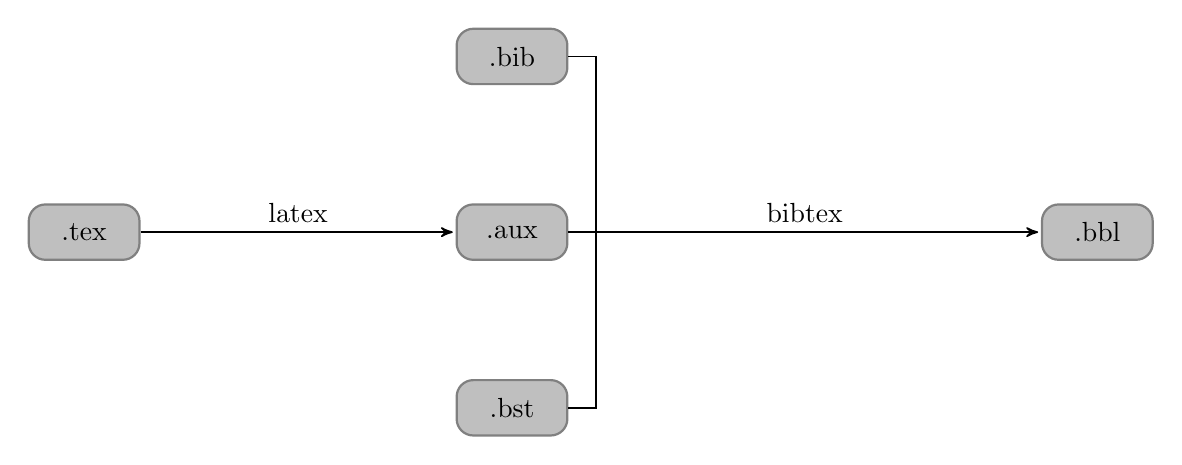
\begin{tikzpicture}
    \node[box] (tex) {.tex};
    \node[box, right=4 of tex] (aux) {.aux};
    \node[box, right=6 of aux] (bbl) {.bbl};
    \node[box, above=1.5 of aux] (bib) {.bib};
    \node[box, below=1.5 of aux] (bst) {.bst};
    \path (tex) edge [arrow] node[auto] {latex} (aux)
        (aux) edge [arrow] node[auto] {bibtex} (bbl)
        (bib.east) edge [rloop] (bst);
\end{tikzpicture}
\caption{\BibTeX~的编译}
\label{fig:bibtex}
\end{figure}

注意在长文档中使用参考文献时,应该用~\verb|latex|~编译主控文档,而用~\verb|bibtex|~编译子文档。

\begin{code}
latex master(.tex)
bibtex chapter1(.tex)
latex master(.tex)
latex master(.tex)
\end{code}

\subsection{natbib}
参考文献的引用通常有两种样式:作者-年份和数字。\LaTeX~本身只支持数字样式,而~\verb|natbib|~宏包\citep{Daly_2007}则同时支持这两种样式。

使用~\verb|natbib|~宏包时,我们首先要引用宏包;其次设置文献列表样式和引用样式,每种列表样式都有自己的缺省引用样式,所以后者可选;然后指定参考文献数据库。
\begin{code}
\usepackage{natbib}
...
\begin{document}
\bibliographystyle{plainnat}
\setcitestyle{square,aysep={},yysep={;}}
\bibliography{mybib.bib}
...
\end{document}
\end{code}

\verb|natbib|~提供了三种列表样式:plainnat、abbrvnat、unsrtnat。前两种都是作者-年份样式,文献列表按作者-年份排序,后者会使用一些缩写(比如作者的~first name);unsrtnat~是数字样式,文献列表按引用顺序排序。

\verb|\setcitestyle|~命令可以用来改变引用样式的设置,其选项见~\Fref{tab:citestyle}。

\begin{table}[htbp]
\caption{参考文献引用样式选项}
\label{tab:citestyle}
\centering
\begin{tabular}{ll}
    \toprule
    引用模式            & authoryear、numbers、super \\
    括号                & round、square、open={char},close={char} \\
    引用条目分隔符      & 分号、逗号、citesep={char} \\
    作者年份分隔符      & aysep={char} \\
    共同作者年份分隔符  & yysep={char} \\
    注解分隔符          & notesep={text} \\
    \bottomrule
\end{tabular}
\end{table}

注意在长文档中,每个含参考文献的子文档都需要分别设置列表样式,并指定数据库。

\verb|natbib|~提供了多种引用命令,其中最基本的是~\verb|\citet|~和~\verb|\citep|~,它们在不同引用模式下效果不同。一般不推荐使用~\LaTeX~本身提供的~\verb|\cite|,因为它在作者-年份模式下和~\verb|\citet|~一样,在数字模式下和~\verb|\citep|~一样。

作者-年份模式下引用命令的效果如下。
\setcitestyle{authoryear}
\begin{demo}
参阅\cite{Daly_2007}\\
参阅\citet{Daly_2007}\\
参阅\citep{Daly_2007}
\end{demo}

数字模式下引用命令的效果如下。
\setcitestyle{numbers}
\begin{demo}
参阅\cite{Daly_2007}\\
参阅\citet{Daly_2007}\\
参阅\citep{Daly_2007}
\end{demo}

上标模式下引用命令的效果如下。
\setcitestyle{super}
\begin{demo}
参阅\cite{Daly_2007}\\
参阅\citet{Daly_2007}\\
参阅\citep{Daly_2007}
\end{demo}

另外还有一些引用命令,如~\verb|\citetext、\citenum、\citeauthor|、~\verb|\citeyear|~等,此处不赘述。

\section{索引}
\verb|makeidx|~宏包提供了索引功能。应用它时,我们首先需要在文档序言部分引用宏包,并使用~\verb|makeindex|~命令;其次在正文中需要索引的地方定义索引,注意索引关键字在全文中须保持唯一;最后在合适的地方(一般是文档末尾)打印索引。

\begin{code}
\usepackage{makeidx}
\makeindex
...
\begin{document}
\index{索引关键字}
...
\printindex
\end{document}
\end{code}

当编译含索引的文档时,用户需要执行~\verb|latex、makeindex、latex|~等三次编译操作。

\begin{enumerate}
    \item 第一遍~\verb|latex|~把索引条目写到一个~\verb|.idx|~文件中去。
    \item \verb|makeindex|~把~\verb|.idx|~排序后写到一个~\verb|.ind|~文件中去。
    \item 第二遍~\verb|latex|~在~\verb|\printindex|~命令的地方引用~\verb|.ind|~的内容,生成正确的DVI。
\end{enumerate}

\begin{figure}[htbp]
\centering
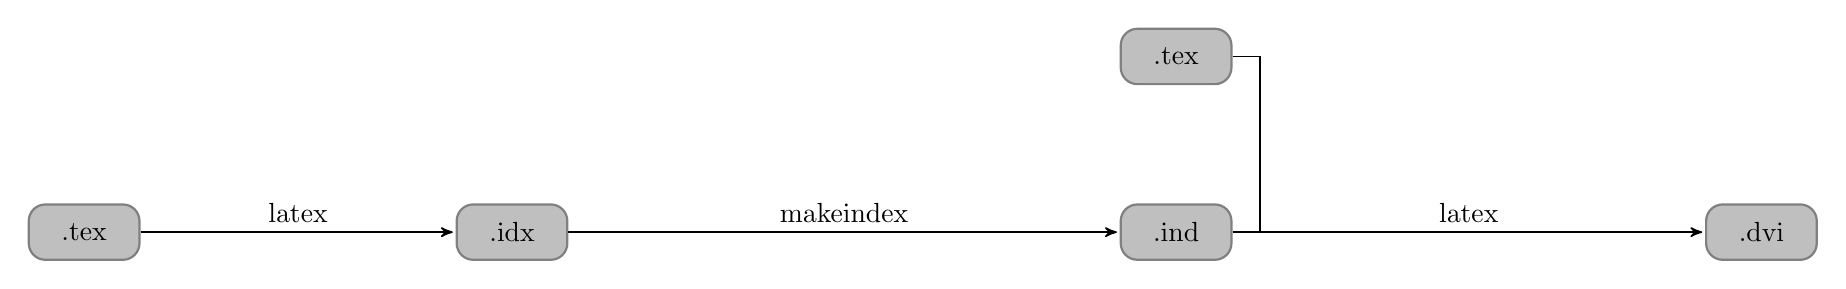
\begin{tikzpicture}
    \node[box] (tex) {.tex};
    \node[box, right=4 of tex] (idx) {.idx};
    \node[box, right=7 of idx] (ind) {.ind};
    \node[box, right=6 of ind] (dvi) {.dvi};
    \node[box, above=1.5 of ind] (tex1) {.tex};
    \node[right=1 of ind] (point) {};
    \path (tex) edge [arrow] node[auto] {latex} (idx)
        (idx) edge [arrow] node[auto] {makeindex} (ind)
        (ind) edge [arrow] node[auto] {latex} (dvi)
        (tex1.east) edge [rloop] (point);
\end{tikzpicture}
\caption{索引的编译}
\label{fig:makeidx}
\end{figure}

\section{页面布局}
在~\LaTeX~中用户可以通过~\verb|\pagestyle|~和~\verb|\pagenumbering|~命令来设置页眉(header)、页脚(footer)的样式和内容。页面样式有以下四种。

\begin{table}[htbp]
\caption{\LaTeX~页面样式}
\centering
\begin{tabular}{ll}
    \toprule
    \texttt{empty} & 页眉、页脚空白 \\
    \texttt{plain} & 页眉空白,页脚含居中页码 \\
    \texttt{headings} & 页脚空白,页眉含章节名和页码 \\
    \texttt{myheadings} & 页脚空白,页眉含页码和用户自定义信息 \\
    \bottomrule
\end{tabular}
\end{table}

\verb|fancyhdr|\citep{Oostrum_2004}宏包提供了更灵活的控制。我们可以用以下代码定制页眉、页脚的内容,以及页眉下方、页脚上方的横线。

\begin{code}
\usepackage{fancyhdr}
...
\pagestyle{fancy} %fancyhdr宏包新增的页面风格
\lhead{左擎苍}
\chead{三个代表}
\rhead{右牵黄}
\lfoot{左青龙}
\cfoot{八荣八耻}
\rfoot{右白虎}
\renewcommand{\headrulewidth}{0.4pt}
\renewcommand{\footrulewidth}{0.4pt}
\end{code}

\ \\
\begin{tikzpicture}
\draw (0,0) rectangle (36,10);
\node at(2,9) {左擎苍};
\node at(18,9) {三个代表};
\node at(34,9) {右牵黄};
\draw (.5,8)--(35.5,8);
\node at(18,5) {和谐社会};
\draw (.5,2)--(35.5,2);
\node at(2,1) {左青龙};
\node at(18,1) {八荣八耻};
\node at(34,1) {右白虎};
\end{tikzpicture}

用户可以在页眉、页脚中使用一些~\LaTeX~变量,比如分别代表页码和章节编号的~\verb|\thepage、\thechapter、\thesection|;代表章节起始单词(Chapter、Section等)的~\verb|\chaptername、\sectionname|~等。

这些变量组合起来可以构成复合标记~\verb|\leftmark|~和~\verb|\rightmark|~。当文档奇偶页面布局不同时,我们可以使用以下方法为奇偶页分别设置页眉、页脚。\verb|fancyhdr|~宏包会自动把每章起始页的样式设为~\verb|plain|,若想去掉页脚中间的页码,可以重定义~\verb|plain|~样式。

\begin{code}
\pagestyle{fancy}
\fancyhf{}                  %清空页眉页脚
\fancyhead[LE,RO]{\thepage} %偶数页左,奇数页右
\fancyhead[RE]{\leftmark}   %偶数页右
\fancyhead[LO]{\rightmark}  %奇数页左
\fancypagestyle{plain}{     %重定义plain页面样式
    \fancyhf{}
    \renewcommand{\headrulewidth}{0pt}
}
\end{code}

\ \\
\begin{tikzpicture}
\draw (0,0) rectangle (36,10);
\node at(2.5,9) {3.2 节名};
\node at(35,9) {17};
\draw (.5,8)--(35.5,8);
\node at(18,5) {奇数页};
\end{tikzpicture}

\ \\
\begin{tikzpicture}
\draw (0,0) rectangle (36,10);
\node at(1,9) {18};
\node at(32,9) {Chapter 3 章名};
\draw (.5,8)--(35.5,8);
\node at(18,5) {偶数页};
\end{tikzpicture}

Lamport当初设计~\LaTeX~时把页面布局变量的定义方式搞得比较晦涩,用户在重定义~\verb|\leftmark|~和~\verb|\rightmark|~时,不能直接用~\verb|\renewcommand|~的方法,而要用另外两个命令。

\begin{code}
\markboth{main-mark}{sub-mark}
\markright{sub-mark}
\end{code}

\verb|\leftmark|~即~main-mark,是一种高层次标记,在~article~文档类中它包含~section~的信息,在~report~和~book~则包含~chapter~的信息;\verb|rightmark|~则是一种低层次标记,在~article~中包含~subsection~信息,在~report~和~book~中包含~section~信息。

比如在~\verb|book|~文档类中,章节标记是通过下面的方法定义的,其中的~\verb|#1|~指的是章节的名字。

\begin{code}
\renewcommand\chaptermark[1]{\markboth{\chaptername \thechapter. 
    #1}{}}
\renewcommand\sectionmark[1]{\markright{\thesection. #1}}
\end{code}

%\section{演示文档}

\bibliographystyle{unsrtnat}
\bibliography{reading}
\newpage

\chapter{中文}

\section{字符集和编码}
\label{sec:encoding}

众所周知电脑内部采用二进制编码,因为它易于用电子电路实现。所有字符(包括字母、数字、符号、控制码等)在电脑内部都是用二进制表示的,字符集(Character Set)的二进制编码被称为字符编码(Character Encoding),有时人们也会混用这两个术语。

1963~年发布的~American Standard Code for Information Interchange(~ASCII)是最早出现的字符编码,它用~7~位(bit)表示了~$2^7=128$个字符,只能勉强覆盖英文字符。

美国人发明了电脑,英语被优先考虑是很自然的事情。随着电脑技术的传播,人们呼吁把字符编码扩充到~8~位也就是一个字节(byte),于是国际标准化组织(International Organization for Standardization,ISO)推出了~ISO 8859。$2^8=256$个字符显然也不能满足需要,所以~8859~被分为十几个部分,从~8859-1(西欧语言)、8859-2(中欧语言),直到~8859-16(东南欧语言),覆盖了大部分使用拉丁字母的语言文字。

在~ISO~标准完全定型之前,IBM~就有一系列自己的字符编码,他们称之为代码页(Code Page),其中著名的有~1981~年就被用于~IBM PC~的~437(扩展~ASCII)、850(西欧语言)、852(东欧语言)。IBM~代码页通常被用于控制台(Console)环境,也就是~MS-DOS~或~Unix Shell~那样的命令行环境。

微软将~IBM~代码页称为~OEM~代码页,自己定义的称为~ANSI~代码页,后者中著名的有1252(西欧语言)、1250(东欧语言)、936(GBK~简体中文)、950(Big5~繁体中文)、932(SJIS~日文)、949(EUC-KR~韩文)等。

1981~年,中国大陆推出了第一个自己的字符集标准~GB2312,它是一个~$94*94$~的表,包括~7445~个字符(含~6763~个汉字)。GB2312~通常采用双字节的EUC-CN编码,所以后者也常常被称为~GB2312~编码;其实~GB2312~还有另一种编码方式~HZ,只是不常用。GB2312~不包含朱镕基的“镕”字,政府、新闻、出版、印刷等行业和部门在使用中感到十分不便,于是它在~1993~年被扩展为~GBK,后者包括~21886~个字符(含~21003~个汉字),没有形成正式标准。2000~年发布的~GB18030~包含~70244~个字符(含~27533~个汉字),采用四字节编码。GB18030~之前还出现过一个~GB13000,没有形成气候。

1990~年ISO~推出了通用字符集(Universal Character Set,UCS),即~ISO 10646,意图一统江湖。它有两种编码:双字节的~UCS-2~和四字节的~UCS-4。

ISO~之外还有个希望一统江湖的组织:统一码联盟(The Unicode Consortium),它于~1991~年推出了~Unicode 1.0。后来两家组织意识到没必要做重复工作,于是开始合并双方的成果,携手奔小康。从~Unicode 2.0~开始,Unicode~采用了与~ISO 10646-1~相同的编码。

Unicode~主要有三种编码:UTF-8、UTF-16、UTF-32。UTF-8~使用一至四个~8~位编码。互联网工程任务组(Internet Engineering Task Force,~IETF)要求所有网络协议都支持~UTF-8,互联网电子邮件联盟(Internet Mail Consortium,IMC)也建议所有电子邮件软件都支持~UTF-8,所以它已成为互联网上的事实标准。UTF-16~用一或两个~16~位编码,基本上是~UCS-2~的超集,和~ASCII~不兼容。UTF-32~用一个~32~位编码,它是~UCS-4~的一个子集。

\section{中文解决方案}
\TeX~是基于单字节编码的,因为~Knuth~当初开发~\TeX~时没考虑那么远,也没有现成的标准可以借鉴。

\LaTeX~对中文的支持主要有两种方法:张林波\footnote{中科院计算数学所某实验室主任。}开发的~\href{ftp://ftp.cc.ac.cn/pub/cct/}{CCT}~和~Werner Lemberg\footnote{1968~年生于奥地利,从维也纳音乐学院获得作曲、指挥、钢琴、乐团管理、歌手教练等五个专业文凭,后自学中文和数学。曾任职于奥地利和德国多家剧院和乐团,现任德国科布伦茨某剧院指挥。}开发的~CJK~宏包。早期~CCT~比较流行,新的~CCT~也可以和~CJK~配合使用,网上可以找到的最后更新是~2003~年的。CJK~是当前主流,它不仅支持中日韩等东亚文字,还支持几十种其他不同语言的多种编码。

支持简体中文的~\LaTeX~发行版有吴凌云\footnote{中科院应用数学所研究员。}的~CTeX~和李树钧\footnote{德国哈根函授大学研究员。}的~ChinaTeX,繁体中文的有吴聪敏\footnote{台湾大学电机系学士,美国罗彻斯特大学经济学博士,现任台湾大学经济系教授。}、吴聪慧兄弟的~cwTeX~和蔡奇伟\footnote{美国犹他大学计算机博士,现任台湾静宜大学资讯工程系教授。}的~PUTeX。后面两个台湾的发行版包老师不熟悉,前面两个大陆的发行版都包含~MikTeX、CCT、CJK、WinEdt~等。

\section{CJK的使用}
CJK~的作者写的使用说明比较凌乱和晦涩,读者可以参阅李果正的《我的CJK》\citep{Lee_2004a}。

CJK~有两个基本宏包:\verb|CJK|~和~\verb|CJKutf8|,后者面向~UTF-8~编码。CJK~环境的一般使用方法如下:

\begin{code}
\usepackage{CJK(utf8)}
...
\begin{document}
\begin{CJK}{<encoding>}{<family>}
...
\end{CJK}
\end{document}
\end{code}

简体中文常用编码是~GBK~和~UTF8~。family~是指宋体、楷体、隶书等,具体引用要看电脑上安装了什么字体。麻烦的是~GBK~和~UTF8~字体不通用,也就是说每种编码需要自己的字体。CJK~自带的~UTF8~简体字体有~gbsn(宋体)和~gkai(楷体)。CTeX~提供的~GBK~字体有~song(宋体)、fs(仿宋)、kai(楷体)、hei(黑体)、li(隶书)、~you(幼圆)等。

注意使用~\verb|CJKutf8|~宏包时,\verb|CJK|~环境的编码最好是~UTF8,否则可能遭遇不测。

下面是一个简单的~GBK~示例和一个~UTF8~示例,注意用编辑器保存时要选则相应的编码格式,比如前者用~ANSI,后者用~UTF-8。
\begin{code}
\documentclass{article}
\usepackage{CJK}
\begin{document}
\begin{CJK}{GBK}{song}
这是一个CJK例子,使用了GBK编码和song字体。
\end{CJK}
\end{document}
\end{code}

\begin{code}
\documentclass{article}
\usepackage{CJKutf8}
\begin{document}
\begin{CJK}{UTF8}{gbsn}
这是一个CJK例子,使用了UTF-8编码和gbsn字体。
\end{CJK}
\end{document}
\end{code}

\bibliographystyle{unsrtnat}
\bibliography{reading}
\newpage

\chapter{字体}

关于字体有三个重要概念:glyph、typeface、font。glyph~通常被翻译为字形,也有翻译为字体的;typeface~是一个书法和印刷领域的概念,它通常被翻译为字体或书体;font~曾经和~typeface~混用,但现在一般用作电脑领域的概念,在中国大陆被翻译为字体,在台湾被翻译为字型。

上述翻译的混乱令人十分无奈,包老师决定在本文中把它们分别翻译为字形、字样、字体,以正视听。

字形是一个字符的具体图形表现形式,一个字符可以有多个字形,比如汉字中的“強/强”、“戶/户/戸”;字样是一组相同风格样式的字形的集合,比如中文字样有宋、仿、楷、黑、隶、篆等;一种字样可以对应电脑上的几种字体。

\section{字样}
\label{sec:typeface}
拉丁字母的字样主要有三大类:Serif(Roman)、Sans Serif~和~Mono-space~(Typewriter)。Serif~的笔画边缘部分有些装饰,类似于中文的宋体、仿宋、楷体、魏书等。Sans Serif~的笔画则是平滑的,类似于中文的黑体。Sans~这个词来源于法语,就是“没有”的意思。Monospace~则是等宽字样。

每一类字样都可以有加粗(bold)、斜体(italic)、倾斜(oblique)等修饰效果。Italic~通常对原字样进行过重新设计,它修饰精细,多用于~Serif;~Oblique~也称作~slanted,基本上是把正体倾斜,多用于~Sans Serif。通常~oblique~看起来比~italic~要宽一些。

\Fref{tab:typeface}列出了几种常见的字样。

\begin{table}[htbp]
\caption{常见字样}
\label{tab:typeface}
\centering
\begin{tabular}{llll}
    \toprule
    操作系统 & Serif           & Sans Serif & Monospace \\
    \midrule
    Mac OS   & Times           & Helvetica  & Courier \\
    Windows  & Times New Roman & Arial      & Courier New \\
    \bottomrule
\end{tabular}
\end{table}

\section{字体格式}
\label{sec:font}

\subsection{点阵字体和矢量字体}
电脑上用的字体(font)按数据格式可以分为三大类:点阵字体(bitmap)、轮廓(outline)字体和笔画(stroke-based)字体。

点阵字体通过点阵来描述字形。早期的电脑受到容量和绘图速度的限制,多采用点阵字体。点阵字体后来渐渐被轮廓字体所取代,但是很多小字号字体仍然使用它,因为这种情况下轮廓字体缩放太多会导致笔画不清晰。

轮廓字体又称作矢量字体,它通过一组直线段和曲线来描述字形。轮廓字体易于通过数学函数进行缩放等变换,形成平滑的轮廓。轮廓字体的主要缺陷在于它所采用的贝塞尔曲线(Bézier curves)在光栅(raster)设备(比如显示器和打印机)上不能精确渲染,因而需要额外的补偿处理比如字体微调(font hinting)。但是随着电脑硬件的发展,人们一般不在意它比点阵字体多出的处理时间。

笔画字体其实也是轮廓字体,不过它描述的不是完整的字形,而是笔画。它多用于东亚文字。

\subsection{常见字体}

常见的轮廓字体技术有:Type 1~和~Type 3、TrueType、OpenType、~\MF~等。

Adobe~的~Type 1~和~Type 3~基于~PS,它们采用三次贝塞尔曲线。Type 1~支持微调,它使用一个简化的~PS~子集;Type 3~不支持微调,但它可以使用全部~PS~功能,因此既可以包含轮廓字体也可以包含点阵字体信息。
    
1991~年,Apple~发布了~TrueType,它采用二次贝塞尔曲线。二次曲线处理起来比三次曲线快,但是需要更多的点来描述。所以从~TrueType~到~Type 1的转换是无损的,反之是有损的。1994~年,Apple~着手研究~TrueType~的下一代技术:TrueType GX,它后来演变为Apple Advanced Typography(AAT)。

1996~年,微软和~Adobe~联合发布了~OpenType。它比起~AAT~的优势有:跨平台、开放和易于开发、支持更多的语言比如阿拉伯语。

早在~1984~年~Knuth~就发布了~\MF,它与~TrueType~和~OpenType的区别是,不直接描述字形轮廓,而描述生成轮廓的笔的轨迹。笔的形状可以是椭圆形或多边形,尺寸缩放自如,字形边缘也柔和一些。两种字体可以用同一个~\MF~文件,当然还有不同的参数。\MF~技术如此先进,却没有流行开来。对此~Knuth~解释道,要求一位设计字体的艺术家掌握~60~个参数太变态了,那是用来折磨数学家的。

Type 1~和~Type 3~把字体信息存储在两种文件里:metrics~和~glyph~文件。metrics~文件有~AFM(Adobe font metrics)和~PFM(printer font metrics),glyph~文件有~PFA(printer font ASCII)和~PFB(printer font binary)。~\LaTeX~使用的~metrics~格式是~TFM(TeX Font Metrics)。

TrueType~的文件后缀是~.ttf,OpenType~的是~.ttf~和~.otf。\MF~虽然用矢量图形来定义字形,实际输出的却是一种点阵格式:PK~(packed raster)。

上述字体按技术的先进性,从高到低的排序为:OpenType、~TrueType、Type 1、Type 3、PK,我们应优先选用~OpenType~和~TrueType。

\subsection{合纵连横}
Adobe~收取的~Type 1~专利许可费一度十分昂贵,穷人们只好用免费的~Type 3。为了打破这种垄断,Apple~开发了~TrueType。1991~年~TrueType~发布之后,Adobe随即公开了~Type 1~的规范,~Type 1~字体从贵族堕落为平民,因而流行开来。

1980~年代中后期,Adobe~的大部分盈利来自于~PS~解释器的许可费。面对这种垄断局面,微软和~Apple~联合了起来。微软把买来的~PS~解释器~TrueImage~授权给~Apple,Apple~则把~TrueType~授权给微软。

微软得陇望蜀,又企图获得~AAT~的许可证,未遂。为了打破~Apple~的垄断,微软联合~Adobe~在1996年发布了~OpenType。Adobe~在2002~年末将其字体库全面转向~OpenType。

上面这几出精彩好戏充分展示了商场上的勾心斗角、尔虞我诈,没有永恒的伙伴,只有永恒的利益。但它同时也告诉我们,市场竞争中受益的还是广大的消费者。

\section{字体应用}

PS~支持~Type 1~和~Type 3,而~PDF~除了这两种还支持~TrueType~和~OpenType。\verb|latex|、DVI浏览器、各种~driver~分别采用不同的字体技术。

\subsection{DVI}
\verb|latex|~编译~\LaTeX~源文件生成~DVI~时只需要\verb|.tfm|~文件,因为~DVI~并不包含字形信息,而只包含对字体的引用。DVI~浏览器显示~DVI~时一般使用~PK,它在系统中查找相应的~\verb|.pk|~文件,若找不到就调用~\MF~在后台自动生成。

\subsection{dvips}
缺省情况下,\verb|dvips|~也会查找~\verb|.pk|~,或调用~\MF~自动生成;然后把~PK~转换成包含点阵字体的~Type 3,它的参数~\verb|-D|~可以用来控制该点阵字体的分辨率。用~\verb|ps2pdf|~处理含~Type 3~的~PS~时,输出的自然是含~Type 3~的~PDF。

GSview~在低分辨率下可以很好地渲染~Type 3,Adobe Reader~或~Acrobat~却不能,因为它们使用的~Adobe Type Manager~不支持包含完整~PS~的~Type 3。含~Type 3~的~PDF~看起来会有些模糊,所以应尽量避免使用。

\verb|dvips|~的另一个参数~\verb|-Ppdf|~把~Type 1~嵌入生成的~PS,这样再~\verb|ps2pdf|~就能生成含~Type 1~的~PDF。

\verb|dvips|~不支持真正的(native)TrueType,用户只能把~TrueType~先转成~PK~或~Type 1,这样绕了个弯效果总会打些折扣。

\verb|dvips|~的字体详细使用方法可查阅其手册\citep{Rokicki_2005}第~6~章,此处不赘述。

\subsection{dvipdfm(x)}
\verb|dvipdfm|~支持~PK~和~Type 1,它可以用一个~\verb|t1fonts.map|~文件建立~PK~文件和~Type 1~文件之间的映射,这样生成的~PDF~用的就是~Type 1。\verb|dvipdfm|~也不支持真正的~TrueType。

\verb|dvipdfmx|~通过正确的设置可以使用真正的~TrueType,它对中日韩等东亚文字的支持也较好,所以它对我们来说是~Driver~的首选。

\section{TrueType~字体安装配置}
CJK~自带的~UTF-8~编码字体~gbsn~和~gkai只包含~GB2312~字符集,而~CTeX~只提供~GBK~编码字体,因此中文用户通常需要自己安装配置~UTF-8~编码的~TrueType~字体。

在使用~TrueType~之前,用户通常需要作以下准备工作:
\begin{enumerate}
    \item 用转换程序~\verb|ttf2tfm|~生成~TFM。
    \item 配置字体定义文件~\verb|.fd|。
    \item 配置~\verb|ttf2pk|~,因为~DVI~浏览器和~\verb|dvips|~都会自动调用~\verb|ttf2pk|~来生成~PK。
    \item 配置~\verb|dvipdfmx|。
\end{enumerate}

\subsection{目录和文件}
通常每个发行包都会参照~TDS~建立自己的目录系统,把各种文件发在固定的位置。比如~MiKTeX~顶层目录如下,在本节后面的示例中我们将使用这些目录的缩写。
\begin{code}
Install: D:\edit\MiKTeX 2.7
UserData: C:\Documents and Settings\Alpha\Local Settings\
    Application Data\MiKTeX\2.7
UserConfig: C:\Documents and Settings\Alpha\
    Application Data\MiKTeX\2.7
\end{code}

目录多了有个缺点,文件不知道放在哪里好。MiKTeX~中有的配置文件居然在四个目录下各有一份,实在是令人发指。幸好我们可以用下面的命令检查配置文件的具体名字和路径。

\begin{code}
initexmf --edit-config-file=ttf2pk
\end{code}

\subsection{ttf2tfm}
比如我们想把~\verb|SimSun18030.ttc|(18030~字符集的新宋体)转换为~UTF8~编码的字体文件,我们需要执行以下步骤。

\begin{enumerate}
    \item 把需要的~\verb|.ttf|~文件复制到~\verb|UserData/fonts/truetype/chinese/|。
    \item 用下面的命令生成\verb|.tfm|~和~\verb|.enc|~文件。
    \item 把~\verb|*.tfm|~复制到~\verb|UserData/fonts/tfm/chinese/utf8song/|。
    \item 把~\verb|*.enc|~复制到~\verb|UserData/fonts/enc/chinese/utf8song/|。
\end{enumerate}

\begin{code}
ttf2tfm SimSun18030.ttc -q -w utf8song@Unicode@
\end{code}

\subsection{字体定义文件}
字体定义文件将字体引用名和实际的字体文件联系起来,比如我们在~\verb|CJK|~环境中引用~\verb|usong|~时,系统将会找到并使用~\verb|utf8song*.tfm|。

\begin{code}
%UserData\tex\latex\CJK\UTF8\C70usong.fd
\ProvidesFile{c70usong.fd}
%character set: GB18030
%font encoding: Unicode
\DeclareFontFamily{C70}{usong}{\hyphenchar \font\m@ne}
\DeclareFontShape{C70}{usong}{m}{n}{<-> CJK * utf8song}{}
\DeclareFontShape{C70}{usong}{m}{it}{<-> CJK * utf8song}{}
\DeclareFontShape{C70}{usong}{bx}{n}{<-> CJKb * utf8song}{
    \CJKbold}
\endinput
\end{code}

\subsection{配置~\texttt{ttf2pk}}
MiKTeX~中~\verb|ttf2pk|~的配置文件是~\verb|ttf2pk.ini|~,在其它的发行包中可能是~\verb|ttf2pk.cfg|。

\verb|ttf2pk.ini|~中有一个~\verb|.map|~文件列表,后者定义了~TrueType~应该按编码转为~PK~等信息。

比如下面这个文件列表会让~\verb|ttf2pk|~读取~\verb|foo.map|~和~\verb|bar.map|。

\begin{code}
map foo.map
map bar.map
\end{code}

如果系统找不到~\verb|ttf2pk.ini|,它会缺省使用~\verb|ttfonts.map|。
\begin{code}
%UserData\ttf2tfm\base\ttfonts.map
utf8song@Unicode@ SimSun18030.ttc
\end{code}

\subsection{配置~\texttt{dvipdfmx}}
配置~\verb|dvipdfmx|~是为了让~PDF~正确地嵌入~TrueType,否则生成的文件中的内容不能复制、粘贴。

\begin{code}
%UserConfig\dvipdfm\config\dvipdfmx.cfg
f cid-x.map
\end{code}

\begin{code}
%UserData\dvipdfm\config\cid-x.map
utf8song@Unicode@ unicode SimSun18030.ttc
\end{code}

\bibliographystyle{unsrtnat}
\bibliography{reading}
\newpage


\backmatter
\chapter{跋}

首先向一路披荆斩棘看到这里的读者表示祝贺,至少在精神上你已经成为一名合格的~\LaTeX{}er。从此你生是~\LaTeX~的人,死是~\LaTeX~的鬼。Once Black, never back。没有坚持到这里的同学自然已经重新投向“邪恶”的~MS Word,毕竟那里点个按钮就可以插入图形,点个下拉框就可以选择字体。

当然~\LaTeX{}er也有简单的出路,就是只使用缺省设置,尽量少用插图;不必理会点阵、矢量,也不必理会~Type 1、Type 3、TrueType、OpenType。因为内容高于形式,你把文章的版面、字体搞得再漂亮,它也不会因此成为《红楼梦》;而《红楼梦》即使是手抄本,也依然是不朽的名著。

包老师曾经以为~\LaTeX~和~Word~的关系就好像是《笑傲江湖》中华山的气宗和剑宗,头十年剑宗进步快,中间十年打个平手,再往后气宗就遥遥领先。至于令狐冲的无招胜有招,风清扬的神龙见首不见尾又是另一重境界,普通人恐怕只能望其颈背。

费尽九牛二虎之力熬到本文杀青的时候,才发现从前的想法很傻很天真。让我们挥一挥衣袖,不带走一片云,卧薪尝胆忍辱负重,耐心等待~\XeTeX~和~Lua\TeX。

%chapter*{索引}
%\printindex

\newpage

\end{CJK*}

\end{document}